

\subsection{4-((2,4-Diaminopyrimidin-5-yl)methyl)-2,6-dimethoxyphenol \compound{cmpd:HOTri}}

%LMO-1-068

\begin{scheme}[H]
	\begin{center}
		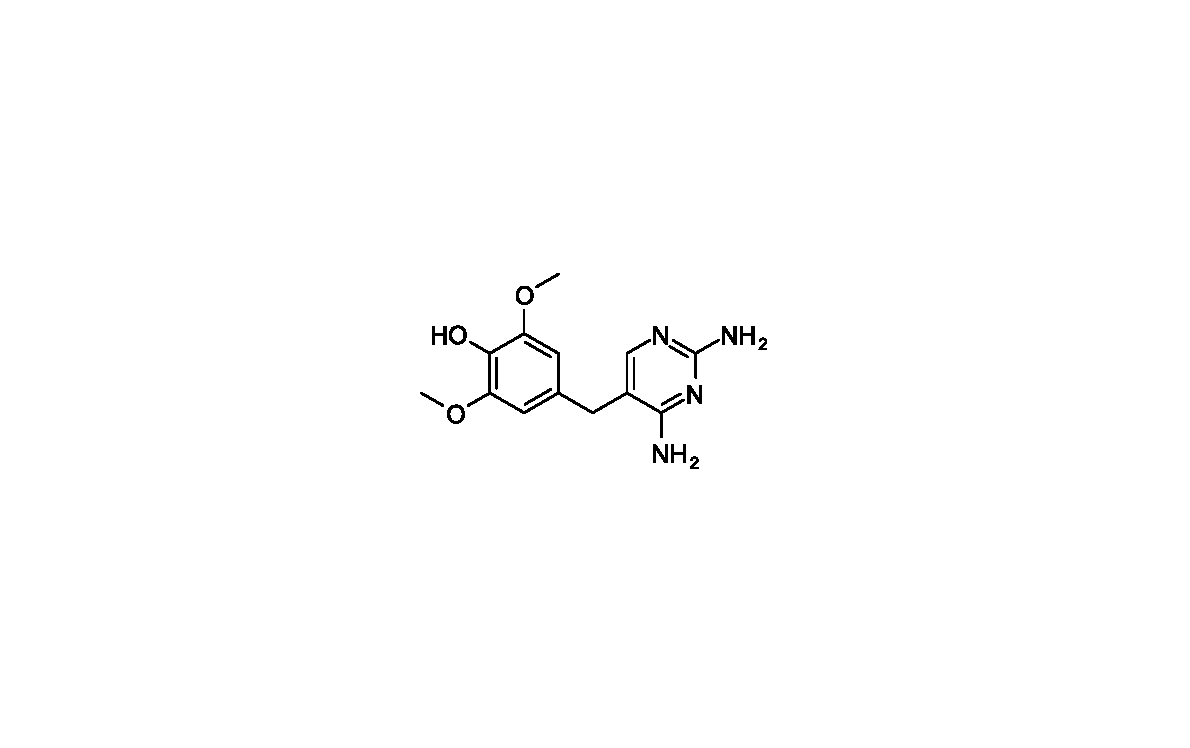
\includegraphics[scale=1]{HOTri}
	\end{center}
\end{scheme}

Hydrobromic acid (48 \% w/w, aq., 50 ml) was heated to 100 $^{\circ}$C. Trimethoprim \compound{cmpd:Tri} (5.00 g, 17.2 mmol) was added, and the suspension was stirred for 40 min under Ar. The mixture was removed from the heat, and NaOH (50 \% w/w, aq., 15 ml) was added dropwise. The reaction mixture was then cooled slowly to 0 $^{\circ}$C, and the resulting crystals were filtered out and washed with cold water. The crystals were then dissolved in hot water (80 ml), neutralized with \ce{NH4OH} (sat., aq.) and cooled slowly to 0 $^{\circ}$C. The resulting crystals were filtered out, washed with cold water and dried under vacuum. \compound{cmpd:HOTri} was obtained as pale pink prisms (2.06 g, 7.46 mmol, 43.4 \%).
\\[1\baselineskip]
\noindent{\textbf{TLC} \textit{R$_f$} = 0.04 (5 \% MeOH/\ce{CHCl2})}
\\[1\baselineskip]
\noindent{\textbf{mp} \textit{T} / $^{\circ}$C = 238 (\ce{H2O}, decomposes)}
\\[1\baselineskip]
\noindent{\textbf{IR} (neat) $\nu_{max}$ / cm$^{-1}$ =
	3314.0 (N-H),
	3137.4 (N-H),
	3045.3 (C-H),
	3000.9 (C-H),
	2938.1 (C-H),
	2838.7 (C-H),
	1662.9 (pyrimidine),
	1645.2 (pyrimidine),
	1626.6 (pyrimidine)}
\\[1\baselineskip]
\noindent{\textbf{$^{1}$H NMR} (400 MHz, MeOD) $\delta$ / ppm = 
	7.21 (s, 1 H, C\underline{H}N), 
	6.54 (s, 2 H, \textit{meta} to OCH$_2$), 
	4.87 (br s, 5 H, OH, NH$_2 \times 2$), 
	3.82 (s, 6 H, OC\underline{H}$_3$), 
	3.63 (s, 2 H, CC\underline{H}$_2$C)}
\\[1\baselineskip]
\noindent{\textbf{$^{13}$C NMR} (101 MHz, MeOD) $\delta$ / ppm = 
	166.4 (CH$_2$C\underline{C}NH$_2$), 
	162.0 (CHN\underline{C}NH$_2$), 
	156.2 (\underline{C}HNCNH$_2$), 
	149.8 (\textit{ipso} to OCH$_3$), 
	135.9 (\textit{ipso} to OH), 
	128.2 (\textit{para} to OH), 
	111.7 (CH$_2$\underline{C}CNH$_2$), 
	107.5 (\textit{meta} to OH), 
	57.0 (O\underline{C}H$_3$), 
	33.9 (C\underline{C}H$_2$C)}
\\[1\baselineskip]
\noindent{\textbf{HRMS} (ESI$^+$) \textit{m}/\textit{z} / Da = 277.1295, [M+H]$^+$ found, [\ce{C13H17N4O3}]$^+$ requires 277.1301}
\\[1\baselineskip]
The data are consistent with the literature\cite{Jing2013}.

%1H NMR (400 MHz, CD3OD) δ ppm: 7.18 (s, 1H), 6.53 (s, 2H), 3.81 (s, 6H), 3.62 (s, 2H). 
%13C NMR (400 MHz, CD3OD) δ ppm: 163.45, 156.58, 148.88, 135.25, 130.78, 107.16, 106.90, 56.50, 33.98. HRMS (FAB+) m/z Calcd. for C13H16O3N4 [M+H]+:277.1222. Found:277.1312.

\subsection{5-(4-(Hex-5-yn-1-yloxy)-3,5-dimethoxybenzyl)pyrimidine-2,4-diamine \compound{cmpd:Y4Tri}}

%LMO-1-069

\begin{scheme}[H]
	\begin{center}
		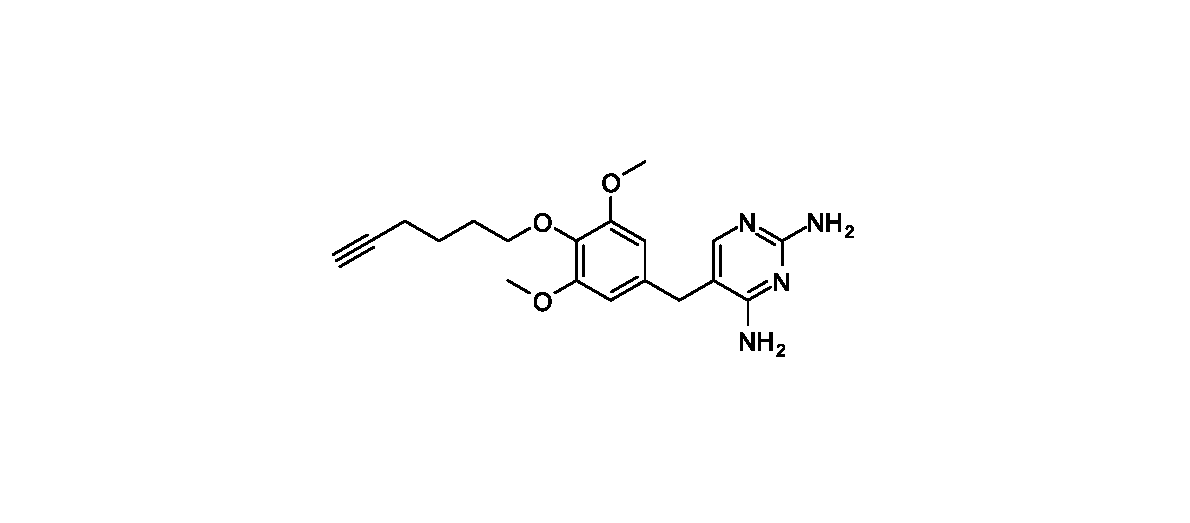
\includegraphics[scale=1]{Y4Tri}
	\end{center}
\end{scheme}

4-((2,4-Diaminopyrimidin-5-yl)methyl)-2,6-dimethoxyphenol \compound{cmpd:HOTri} (1.00 g, 3.62 mmol, 1 eq.), 6-chloro-1-hexyne \compound{cmpd:Y4Cl} (0.524 ml, 0.420 g, 4.34 mmol, 1.2 eq.), \ce{Cs2CO3} (2.36 g, 7.24 mmol, 2 eq.) and anhydrous DMF (30 ml) were stirred at 70 $^{\circ}$C for 7 h. The solvent was removed under reduced pressure, then \ce{CH2Cl2} (30 ml) was added and the mixture filtured. The filtrate was concentrated under reduced pressure and purified by column chromatography using a Combiflash (\ce{SiO2}, 5 \% MeOH/\ce{CH2Cl2}). \compound{cmpd:Y4Tri} was obtained as a pale cream amorphous solid (0.327 g, 0.917 mmol, 25.3 \%).
\\[1\baselineskip]
\noindent{\textbf{TLC} \textit{R$_f$} = 0.14 (5 \% MeOH/\ce{CH2Cl2})}
\\[1\baselineskip]
%\noindent{\textbf{mp} \textit{T} / $^{\circ}$C = ?? (??)}
%\\[1\baselineskip]
\noindent{\textbf{IR} (neat) $\nu_{max}$ / cm$^{-1}$ = 
	3451.4 (alkyne C-H),
	3313.4 (N-H),
	3136.7 (N-H),
	3113.9 (N-H),
	2944.2 (C-H),
	2839.0 (C-H),
	1635.1 (pyrimidine)}
\\[1\baselineskip]
\noindent{\textbf{$^{1}$H NMR} (400 MHz, MeOD) $\delta$ / ppm = 
	7.77 (s, 1 H, C\underline{H}N), 
	6.37 (s, 2 H, \textit{meta} to OCH$_2$), 
	4.83 (br s, 2 H, CHNCN\underline{H}$_2$), 
	4.63 (br s, 2 H, CH$_2$CCN\underline{H}$_2$), 
	3.95 (t, \textit{J} = 6.3 Hz, 2 H, C\underline{H}$_2$O), 
	3.79 (s, 6 H, OC\underline{H}$_3$), 
	3.65 (s, 2 H, CC\underline{H}$_2$C), 
	2.28 (td, \textit{J} = 7.1, 2.6 Hz, 2 H, HC$\equiv$CC\underline{H}$_2$), 
	1.94 (t, \textit{J} = 2.7 Hz, 1 H, \underline{H}C$\equiv$C), 
	1.81 - 1.90 (m, 2 H, C\underline{H}$_2$CH$_2$O), 
	1.71 - 1.80 (m, 2 H, C\underline{H}$_2$CH$_2$CH$_2$O)}
\\[1\baselineskip]
\noindent{\textbf{$^{13}$C NMR} (101 MHz, MeOD) $\delta$ / ppm = 
	162.7 (CH$_2$C\underline{C}NH$_2$), 
	162.0 (CHN\underline{C}NH$_2$), 
	156.4 (\underline{C}HNCNH$_2$), 
	153.8 (\textit{ipso} to OCH$_3$), 
	136.0 (\textit{ipso} to OCH$_2$), 
	133.6 (\textit{para} to OCH$_2$), 
	106.5 (CH$_2$\underline{C}CNH$_2$), 
	105.0 (\textit{meta} to OCH$_2$), 
	84.5 (HC$\equiv$\underline{C}), 
	72.6 (\underline{C}H$_2$O), 
	68.3 (H\underline{C}$\equiv$C), 
	56.1 (O\underline{C}H$_3$), 
	34.7 (C\underline{C}H$_2$C), 
	29.1 (\underline{C}H$_2$CH$_2$O), 
	24.9 (\underline{C}H$_2$CH$_2$CH$_2$O), 
	18.0 (HC$\equiv$C\underline{C}H$_2$)}
\\[1\baselineskip]
\noindent{\textbf{HRMS} (ESI$^+$) \textit{m}/\textit{z} / Da = 357.1920, [M+H]$^+$ found, [\ce{C19H25N4O3}]$^+$ requires 357.1927}
\\[1\baselineskip]
The compound has not been reported previously.

\subsection{Optimised general procedure for the click reaction \label{sec:click_general}}

Azide (1 eq.) and alkyne (1 eq.) were dissolved in 50 \% \textit{t}-BuOH/water in a round-bottomed flask with a stirrer bar, closed with a new septum. The mixture was degassed by bubbling through \ce{N2}. The mixture was placed under positive pressure of Ar using a balloon. 
Equimolar amounts of \ce{CuSO4.5H2O} and THPTA \compound{cmpd:THPTA} were dissolved in water to make a 50 mM solution and similarly degassed.
Sodium ascorbate was dissolved in water to make a 100 mM solution and similarly degassed.
The Cu/THPTA solution (0.05 eq.) was added to the reaction mixture, followed by the sodium ascorbate solution (0.1 eq.). The mixture was stirred for 2 h and monitored using LCMS.
HL derivative conjugates were dry-loaded onto \ce{SiO2} and purified by column chromatography (\ce{SiO2}, 0-20 \% MeOH/\ce{CH2Cl2}).
Other conjugates were purified by preparative HPLC (5-95 \% acetonitrile (0.1 \% TFA)/water (0.05 \% TFA) over 20 min).

\subsection{(\textit{S})-1-Cyclopropyl-6-fluoro-4-oxo-7-(4-(4-(1-(2-oxo-2-((2-oxotetrahydrofuran\hyp{}3\hyp{}yl)amino)ethyl)-1\textit{H}-1,2,3-triazol-4-yl)butyl)piperazin-1-yl)-1,4-dihydroqui\allowbreak n\allowbreak oline-3-carboxylic acid \compound{cmpd:HL2T4Cip}}
	
%LMO-1-092
	
	\begin{scheme}[H]
		\begin{center}
			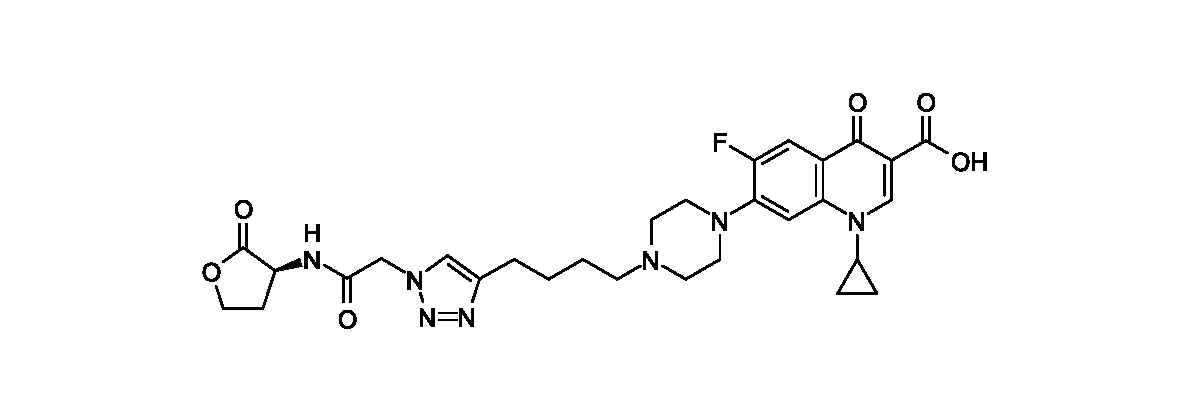
\includegraphics[scale=1]{HL2T4Cip}
		\end{center}
	\end{scheme}

50 \% water/\textit{t}-BuOH (2 ml) was degassed by bubbling \ce{N2} through it. This was then added to a mixture of 1-cyclopropyl-6-fluoro-7-(4-(hex-5-yn-1-yl)piperazin-1-yl)-4-oxo-1,4\hyp{}dihydro\-quinoline-3-carboxylic acid \compound{cmpd:Y4Cip} (20.6 mg, 50.0 $\mu$mol, 1 eq.) and (\textit{S})-2-azido-\textit{N}-(2-oxotetrahydrofuran-3-yl)acetamide \compound{cmpd:HL2N3} (9.2 mg, 50.0 $\mu$mol, 1 eq.).
A similarly degassed solution of \ce{CuSO4.5H2O} (624 $\mu$g, 2.5 $\mu$mol, 0.05 eq. 50 mM), THPTA (1.09 mg, 2.5 $\mu$mol, 0.05 eq. 50 mM) and sodium ascorbate (991 $\mu$g, 5 $\mu$mol, 0.1 eq., 100 mM) in 50 \% water/\textit{t}-BuOH (50 $\mu$l) was then added. 
The mixture was stirred at r.t. under argon for 3 h. On observation that the reaction had stalled, the reaction was degassed again, and a further portion of cataylst solution (50 $\mu$l) was added.
After a further 3 h the reaction mixture was dry-loaded onto \ce{SiO2} and purified by column chromatography using a Combiflash (\ce{SiO2}, 0-20 \% MeOH/\ce{CH2Cl2} over 15 min).
The combined pure fractions were dried with \ce{MgSO4} and evaporated under reduced pressure.
\compound{cmpd:HL2T4Cip} was obtained as a white amorphous solid (8.8 mg, 14.8 $\mu$mol, 29.6 \%).
\\[1\baselineskip]
%\noindent{\textbf{TLC} \textit{R$_f$} = ?? (??)}
%\\[1\baselineskip]
%\noindent{\textbf{mp} \textit{T} / $^{\circ}$C = ?? (??)}
%\\[1\baselineskip]
\noindent{\textbf{IR} (neat) $\nu_{max}$ / cm$^{-1}$ = 
	3266.3 (N-H),
	2949.0 (C-H),
	2934.8 (C-H),
	2827.2 (C-H),
	1778.0 (lactone C=O),
	1724.9 (carboxylic acid C=O),
	1665.0 (amide C=O),
	1625.5 (quinolone C=O)}
\\[1\baselineskip]
\noindent{\textbf{$^{1}$H NMR} (400 MHz, DMSO d$_6$) $\delta$ / ppm = 
	15.23 (s, 1 H, C(=O)O\underline{H}), 
	8.84 (d, \textit{J} = 7.9 Hz, 1 H, N\underline{H}), 
	8.66 (s, 1 H, \textit{ortho} to C(=O)OH), 
	7.90 (d, \textit{J} = 13.3 Hz, 1 H, \textit{ortho} to F), 
	7.82 (s, 1 H, C\underline{H}=CCH$_2$), 
	7.57 (d, \textit{J} = 7.6 Hz, 1 H, \textit{meta} to F), 
	5.13 (s, 1 H, C(=O)C\underline{H}HN),
	5.12 (s, 1 H, C(=O)CH\underline{H}N), 
	4.64 (ddd, \textit{J} = 10.9, 9.0, 7.8 Hz, 1 H, C\underline{H}NH), 
	4.36 (td, \textit{J} = 8.9, 1.7 Hz, 1 H, OC\underline{H}H), 
	4.23 (ddd, \textit{J} = 10.6, 8.8, 6.4 Hz, 1 H, OCH\underline{H}), 
	3.83 (tt, \textit{J} = 7.0, 4.0 Hz, 1 H, NC\underline{H}(CH$_2$)$_2$), 
	3.32 (br s, 4 H, CH$_2$CH$_2$CH$_2$N(CH$_2$C\underline{H}$_2$)CH$_2$C\underline{H}$_2$), 
	2.67 (t, \textit{J} = 7.4 Hz, 2 H, CH=CC\underline{H}$_2$), 
	2.58 (br t, \textit{J} = 5.0 Hz, 4 H, CH$_2$CH$_2$CH$_2$N(C\underline{H}$_2$)C\underline{H}$_2$), 
	2.42 - 2.49 (m, 1 H, OCH$_2$C\underline{H}H), 
	2.40 (t, \textit{J} = 7.1 Hz, 2 H, CH=CCH$_2$CH$_2$CH$_2$C\underline{H}$_2$), 
	2.17 (dtd, \textit{J} = 11.7, 10.8, 9.0 Hz, 1 H, OCH$_2$CH\underline{H}), 
	1.66 (quin, \textit{J} = 7.2 Hz, 2 H, CH=CCH$_2$C\underline{H}$_2$), 
	1.53 (quin, \textit{J} = 7.2 Hz, 2 H, CH=CCH$_2$CH$_2$C\underline{H}$_2$), 
	1.28 - 1.35 (m, 2 H, NCH(C\underline{H}H)$_2$), 
	1.16 - 1.21 (m, 2 H, NCH(CH\underline{H})$_2$)}
\\[1\baselineskip]
\noindent{\textbf{$^{13}$C NMR} (101 MHz, DMSO d$_6$) $\delta$ / ppm = 
	176.4 (\underline{C}(=O)CC(=O)OH), 
	174.9 (O\underline{C}(=O)), 
	166.0 (\underline{C}(=O)OH), 
	165.9 (NH\underline{C}(=O)), 
	153.1 (d, \textit{J} = 250.8 Hz, \textit{ipso} to F), 
	148.0 (\underline{C}H=CC(=O)OH), 
	146.6 (CH=\underline{C}CH$_2$), 
	145.3 (d, \textit{J} = 9.6 Hz, \textit{ipso} to piperazine), 
	139.2 (\textit{para} to F), 
	123.4 (\underline{C}H=CCH$_2$), 
	118.5 (d, \textit{J} = 7.5 Hz, \textit{para} to piperazine), 
	110.9 (d, \textit{J} = 23.5 Hz, \textit{ortho} to C=O and \textit{ortho} to F), 
	106.7 (\underline{C}C(=O)OH), 
	106.4 (d, \textit{J} = 3.2 Hz, \textit{meta} to C=O and \textit{meta} to F), 
	65.4 (O\underline{C}H$_2$), 
	57.3 (CH=CCH$_2$CH$_2$CH$_2$\underline{C}H$_2$N), 
	52.4 (CH$_2$CH$_2$CH$_2$N(\underline{C}H$_2$)\underline{C}H$_2$), 
	51.2 (C(=O)\underline{C}H$_2$N), 
	49.5 (CH$_2$CH$_2$CH$_2$N(CH$_2$\underline{C}H$_2$)CH$_2$CH$_2$), 
	49.5 (CH$_2$CH$_2$CH$_2$N(CH$_2$CH$_2$)CH$_2$\underline{C}H$_2$), 
	48.2 (\underline{C}HNH), 
	35.9 (N\underline{C}H(CH$_2$)$_2$), 
	28.2 (\underline{C}H$_2$CHNH), 
	26.8 (CH=CCH$_2$\underline{C}H$_2$), 
	25.7 (CH=CCH$_2$CH$_2$\underline{C}H$_2$), 
	24.9 (CH=C\allowbreak \underline{C}H$_2$), 
	7.6 (NCH(\underline{C}H$_2$)$_2$)}
\\[1\baselineskip]
%\noindent{\textbf{$^{19}$F NMR} (376.45 MHz, DMSO d$_6$) $\delta$ / ppm = 
%	??
%\\[1\baselineskip]
\noindent{\textbf{HRMS} (ESI$^+$) \textit{m}/\textit{z} / Da = 596.2627, [M+H]$^+$ found, [\ce{C29H35FN7O6}]$^+$ requires 596.2633}
\\[1\baselineskip]
\noindent{[\bm{$\alpha$}]$_D^{20}$ / $^{\circ}$10$^{-1}$cm$^2$g$^{-1}$ = -3.5 (\textit{c} / g(100 ml)$^{-1}$ = 0.0575 , MeOH)}
\\[1\baselineskip]
The compound has not been reported previously.

\subsection{(\textit{S})-1-Cyclopropyl-6-fluoro-4-oxo-7-(4-(4-(1-(4-oxo-4-((2-oxotetrahydrofuran\hyp{}3\hyp{}yl)amino)butyl)-1\textit{H}-1,2,3-triazol-4-yl)butyl)piperazin-1-yl)-1,4-dihydroquin\allowbreak ol\allowbreak ine-3-carboxylic acid \compound{cmpd:HL4T4Cip}}
	
\begin{scheme}[H]
	\begin{center}
		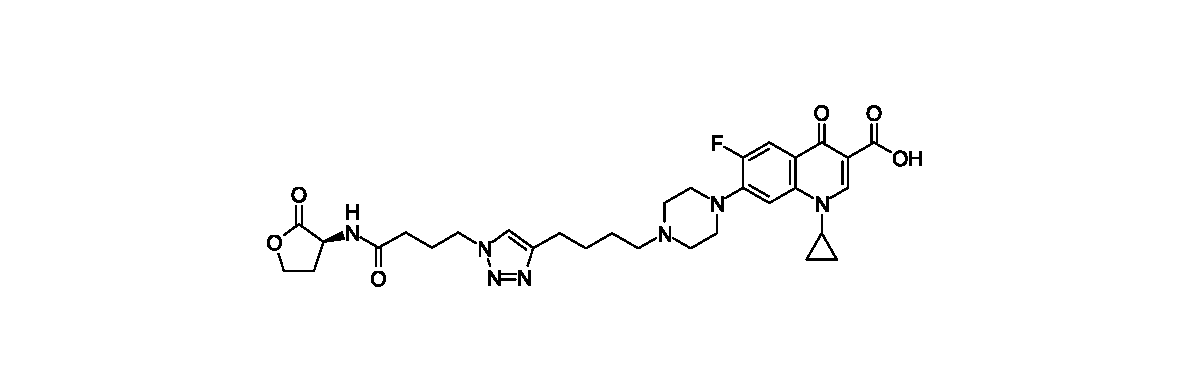
\includegraphics[scale=1]{HL4T4Cip}
	\end{center}
\end{scheme}

%LMO-1-094

50 \% water/\textit{t}-BuOH (2 ml) was degassed by bubbling \ce{N2} through it. This was then added to a mixture of 1-cyclopropyl-6-fluoro-7-(4-(hex-5-yn-1-yl)piperazin-1-yl)-4-oxo-1,4\hyp{}dihydro\-quinoline-3-carboxylic acid \compound{cmpd:Y4Cip} (20.6 mg, 50.0 $\mu$mol, 1 eq.) and (\textit{S})-4-azido-\textit{N}-(2-oxotetrahydrofuran-3-yl)butanamide \compound{cmpd:HL4N3} (10.6 mg, 50.0 $\mu$mol, 1 eq.).
A similarly degassed solution of \ce{CuSO4.5H2O} (624 $\mu$g, 2.5 $\mu$mol, 0.05 eq. 50 mM), THPTA (1.09 mg, 2.5 $\mu$mol, 0.05 eq. 50 mM) and sodium ascorbate (991 $\mu$g, 5 $\mu$mol, 0.1 eq., 100 mM) in 50 \% water/\textit{t}-BuOH (50 $\mu$l) was then added. 
The mixture was stirred at r.t. under argon for 3 h, then dry-loaded onto \ce{SiO2} and purified by column chromatography using a Combiflash (\ce{SiO2}, 0-20 \% MeOH/\ce{CH2Cl2} over 15 min).
The combined pure fractions were dried with \ce{MgSO4} and evaporated under reduced pressure.
\compound{cmpd:HL4T4Cip} was obtained as a white amorphous solid (14.6 mg, 23.4 $\mu$mol, 46.8 \%).
\\[1\baselineskip]
%\noindent{\textbf{TLC} \textit{R$_f$} = ?? (??)}
%\\[1\baselineskip]
%\noindent{\textbf{mp} \textit{T} / $^{\circ}$C = ?? (??)}
%\\[1\baselineskip]
\noindent{\textbf{IR} (neat) $\nu_{max}$ / cm$^{-1}$ = 
	3286.7 (N-H),
	2949.7 (C-H),
	2820.6 (C-H),
	2778.0 (C-H),
	1778.1 (lactone C=O),
	1725.6 (carboxylic acid C=O),
	1663.7 (amide C=O),
	1625.8 (quinolone C=O)}
\\[1\baselineskip]
\noindent{\textbf{$^{1}$H NMR} (500 MHz, DMSO d$_6$) $\delta$ / ppm = 
	15.22 (br s, 1 H, C(=O)O\underline{H}), 
	8.65 (s, 1 H, \textit{ortho} to C(=O)OH), 
	8.40 (d, \textit{J} = 8.0 Hz, 1 H, N\underline{H}), 
	7.88 (d, \textit{J} = 13.4 Hz, 1 H, \textit{ortho} to F), 
	7.85 (s, 1 H, C\underline{H}=CCH$_2$), 
	7.55 (d, \textit{J} = 7.5 Hz, 1 H, \textit{meta} to F), 
	4.53 (ddd, \textit{J} = 10.9, 9.0, 8.1 Hz, 1 H, C\underline{H}NH), 
	4.33 (td, \textit{J} = 8.9, 1.8 Hz, 1 H, OC\underline{H}H), 
	4.31 (t, \textit{J} = 7.0 Hz, 2 H, C\underline{H}$_2$NCH=C), 
	4.20 (ddd, \textit{J} = 10.5, 8.8, 6.5 Hz, 1 H, OCH\underline{H}), 
	3.82 (tt, \textit{J} = 6.9, 4.0 Hz, 1 H, NC\underline{H}(CH$_2$)$_2$), 
	3.32 (br. t, \textit{J} = 4.2 Hz, 4 H, CH$_2$CH$_2$CH$_2$N(CH$_2$C\underline{H}$_2$)CH$_2$C\underline{H}$_2$), 
	2.64 (t, \textit{J} = 7.4 Hz, 2 H, CH=CC\underline{H}$_2$), 
	2.57 (br. t, \textit{J} = 5.0 Hz, 2 H, CH$_2$CH$_2$CH$_2$N(C\underline{H}$_2$)C\underline{H}$_2$), 
	2.34 - 2.42 (m, 3 H, OCH$_2$C\underline{H}H and CH=CCH$_2$CH$_2$CH$_2$C\underline{H}$_2$), 
	2.09 - 2.19 (m, 3 H, OCH$_2$CH\underline{H} and C(=O)C\underline{H}$_2$), 
	2.02 (quin, \textit{J} = 7.2 Hz, 2 H, C(=O)CH$_2$C\underline{H}$_2$), 
	1.64 (quin, \textit{J} = 7.6 Hz, 2 H, CH=CCH$_2$C\underline{H}$_2$), 
	1.52 (quin, \textit{J} = 7.2 Hz, 2 H, CH=CCH$_2$CH$_2$C\underline{H}$_2$), 
	1.29 - 1.34 (m, 2 H, NCH(C\underline{H}H)$_2$), 
	1.15 - 1.21 (m, 2 H, NCH(CH\underline{H})$_2$)}
\\[1\baselineskip]
\noindent{\textbf{$^{13}$C NMR} (126 MHz, DMSO d$_6$) $\delta$ / ppm = 
	176.3 (\underline{C}(=O)CC(=O)OH), 
	175.4 (O\underline{C}(=O)), 
	171.2 (NH\underline{C}(=O)), 
	166.0 (\underline{C}(=O)OH), 
	153.0 (d, \textit{J} = 248.6 Hz, \textit{ortho} to F), 
	148.0 (\underline{C}H=CC(=O)OH), 
	146.8 (CH=\underline{C}CH$_2$), 
	145.2 (d, \textit{J} = 9.6 Hz, \textit{ipso} to piperazine), 
	139.2 (\textit{para} to F), 
	121.7 (\underline{C}H=CCH$_2$), 
	118.5 (d, \textit{J} = 7.5 Hz, \textit{para} to piperazine), 
	110.9 (d, \textit{J} = 22.4 Hz, \textit{ortho} to C=O and \textit{ortho} to F), 
	106.7 (\underline{C}C(=O)OH), 
	106.3 (d, \textit{J} = 3.2 Hz, \textit{meta} to C=O and \textit{meta} to F), 
	65.3 (O\underline{C}H$_2$), 
	57.3 (CH=CCH$_2$CH$_2$CH$_2$\underline{C}H$_2$N), 
	52.4 (CH$_2$CH$_2$CH$_2$N(\underline{C}H$_2$)\underline{C}H$_2$), 
	49.5 (CH$_2$CH$_2$CH$_2$N(CH$_2$\underline{C}H$_2$)CH$_2$CH$_2$), 
	49.4 (CH$_2$CH$_2$CH$_2$N(CH$_2$CH$_2$)CH$_2$\underline{C}H$_2$), 
	48.6 (\underline{C}H$_2$NCH=C), 
	47.9 (OC(=O)\underline{C}HNH), 
	35.9 (N\underline{C}H(CH$_2$)$_2$), 
	31.7 (NHC(=O)\underline{C}H$_2$), 
	28.2 (\underline{C}H$_2$CHNH),  
	26.9 (CH=CCH$_2$\underline{C}H$_2$), 
	25.8 (NHC(=O)CH$_2$\underline{C}H$_2$ and CH=CCH$_2$CH$_2$\underline{C}H$_2$), 
	24.9 (CH=C\underline{C}H$_2$), 
	7.6 (NCH(\underline{C}H$_2$)$_2$)}
\\[1\baselineskip]
%\noindent{\textbf{$^{19}$F NMR} (376.45 MHz, MeOD) $\delta$ / ppm = 
%	??
%\\[1\baselineskip]
\noindent{\textbf{HRMS} (ESI$^+$) \textit{m}/\textit{z} / Da = 624.2928, [M+H]$^+$ found, [\ce{C31H39FN7O6}]$^+$ requires 624.2946}
\\[1\baselineskip]
\noindent{[\bm{$\alpha$}]$_D^{20}$ / $^{\circ}$10$^{-1}$cm$^2$g$^{-1}$ = -10.6 (\textit{c} / g(100 ml)$^{-1}$ = 0.094 , MeOH)}
\\[1\baselineskip]
The compound has not been reported previously.

\subsection{(\textit{S})-1-Cyclopropyl-6-fluoro-4-oxo-7-(4-(4-(1-(6-oxo-6-((2-oxotetrahydrofuran\hyp{}3\hyp{}yl)amino)hexyl)-1\textit{H}-1,2,3-triazol-4-yl)butyl)piperazin-1-yl)-1,4-dihydroquin\allowbreak ol\allowbreak ine-3-carboxylic acid \compound{cmpd:HL6T4Cip}}
	
\begin{scheme}[H]
	\begin{center}
		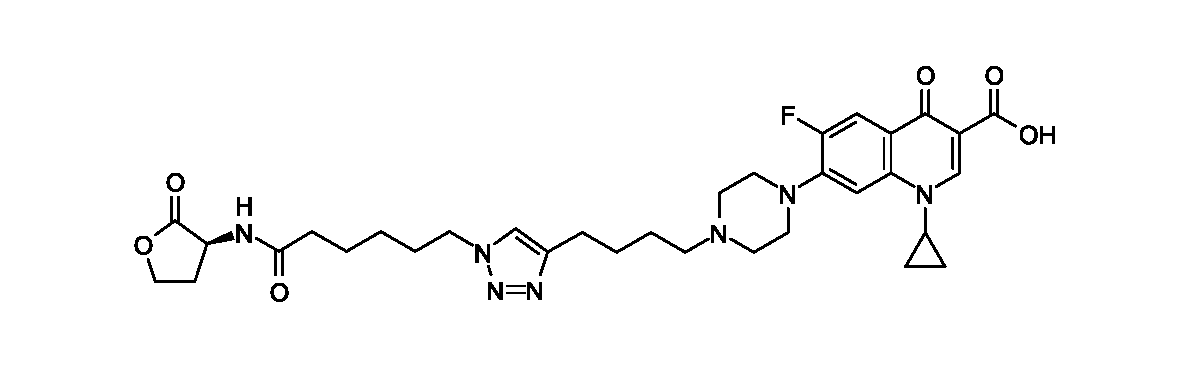
\includegraphics[scale=1]{HL6T4Cip}
	\end{center}
\end{scheme}

%LMO-1-093
	
50 \% water/\textit{t}-BuOH (2 ml) was degassed by bubbling \ce{N2} through it. This was then added to a mixture of 1-cyclopropyl-6-fluoro-7-(4-(hex-5-yn-1-yl)piperazin-1-yl)-4-oxo-1,4\hyp{}dihydro\-quinoline-3-carboxylic acid \compound{cmpd:Y4Cip} (20.6 mg, 50.0 $\mu$mol, 1 eq.) and (\textit{S})-6-azido-\textit{N}-(2-oxotetrahydrofuran-3-yl)hexanamide \compound{cmpd:HL6N3} (12.0 mg, 50.0 $\mu$mol, 1 eq.).
A similarly degassed solution of \ce{CuSO4.5H2O} (624 $\mu$g, 2.5 $\mu$mol, 0.05 eq. 50 mM), THPTA (1.09 mg, 2.5 $\mu$mol, 0.05 eq. 50 mM) and sodium ascorbate (991 $\mu$g, 5 $\mu$mol, 0.1 eq., 100 mM) in 50 \% water/\textit{t}-BuOH (50 $\mu$l) was then added. 
The mixture was stirred at r.t. under argon for 3 h, then dry-loaded onto \ce{SiO2} and purified by column chromatography using a Combiflash (\ce{SiO2}, 0-20 \% MeOH/\ce{CH2Cl2} over 15 min)
The combined pure fractions were dried with \ce{MgSO4} and evaporated under reduced pressure.
\compound{cmpd:HL6T4Cip} was obtained as a white amorphous solid (12.4 mg, 19.0 $\mu$mol, 38.0 \%).
\\[1\baselineskip]
\noindent{\textbf{TLC} \textit{R$_f$} = 0.30 (30 \% MeOH/\ce{CH2Cl2})}
\\[1\baselineskip]
%\noindent{\textbf{mp} \textit{T} / $^{\circ}$C = ?? (??)}
%\\[1\baselineskip]
\noindent{\textbf{IR} (neat) $\nu_{max}$ / cm$^{-1}$ = 
	3301.8 (N-H),
	2939.7 (C-H),
	2857.5 (C-H),
	1784.6 (lactone C=O),
	1728.5 (carboxylic acid C=O),
	1658.2 (amide C=O),
	1625.5 (quinolone C=O)}
\\[1\baselineskip]
\noindent{\textbf{$^{1}$H NMR} (500 MHz, DMSO d$_6$) $\delta$ / ppm = 
	15.22 (br s, 1 H, C(=O)O\underline{H}), 
	8.65 (s, 1 H, \textit{ortho} to C(=O)OH), 
	8.32 (d, \textit{J} = 8.0 Hz, 1 H, N\underline{H}), 
	7.89 (d, \textit{J} = 13.3 Hz, 1 H, \textit{ortho} to F), 
	7.84 (s, 1 H, C\underline{H}=CCH$_2$), 
	7.55 (d, \textit{J} = 7.6 Hz, 1 H, \textit{meta} to F), 
	4.51 (ddd, \textit{J} = 10.9, 9.1, 7.9 Hz, 1 H, C\underline{H}NH), 
	4.33 (td, \textit{J} = 8.8, 1.8 Hz, 1 H, OC\underline{H}H), 
	4.28 (t, \textit{J} = 7.1 Hz, 2 H, C\underline{H}$_2$NCH=C), 
	4.19 (ddd, \textit{J} = 10.5, 8.7, 6.6 Hz, 1 H, OCH\underline{H}), 
	3.82 (tt, \textit{J} = 7.0, 4.0 Hz, 1 H, NC\underline{H}(CH$_2$)$_2$), 
	3.32 (br t, \textit{J} = 4.5, 4 H, CH$_2$CH$_2$CH$_2$N(CH$_2$C\underline{H}$_2$)CH$_2$C\underline{H}$_2$), 
	2.63 (t, \textit{J} = 7.5 Hz, 2 H, CH=CC\underline{H}$_2$), 
	2.57 (br t, \textit{J} = 4.2 Hz, 4 H, CH$_2$CH$_2$CH$_2$N(C\underline{H}$_2$)C\underline{H}$_2$), 
	2.33 - 2.41 (m, 3 H, OCH$_2$C\underline{H}H and CH=CCH$_2$CH$_2$CH$_2$C\underline{H}$_2$), 
	2.06 - 2.16 (m, 3 H, OCH$_2$CH\underline{H} and C(=O)C\underline{H}$_2$), 
	1.79 (quin, \textit{J} = 7.4 Hz, 2 H, C(=O)CH$_2$CH$_2$CH$_2$C\underline{H}$_2$), 
	1.63 (quin, \textit{J} = 7.5 Hz, 2 H, CH=CCH$_2$C\underline{H}$_2$), 
	1.45 - 1.56 (m, 4 H, C(=O)CH$_2$C\underline{H}$_2$ and CH=CCH$_2$CH$_2$C\underline{H}$_2$), 
	1.29 - 1.34 (m, 2 H, NCH(C\underline{H}H)$_2$), 
	1.19 - 1.25 (m, 2 H, C(=O)CH$_2$CH$_2$C\underline{H}$_2$), 
	1.15 - 1.19 (m, 2 H, NCH(CH\underline{H})$_2$)}
\\[1\baselineskip]
\noindent{\textbf{$^{13}$C NMR} (126 MHz, DMSO d$_6$) $\delta$ / ppm = 
	176.4 (\underline{C}(=O)CC(=O)OH), 
	175.4 (O\underline{C}(=O)), 
	172.1 (NH\underline{C}(=O)), 
	166.0 (\underline{C}(=O)OH), 
	153.0 (d, \textit{J} = 250.2 Hz, \textit{ipso} to F), 
	148.0 (\underline{C}H=CC(=O)OH), 
	146.8 (CH=\underline{C}CH$_2$), 
	145.2 (d, \textit{J} = 9.6 Hz, \textit{ipso} to piperazine), 
	139.2 (\textit{para} to F), 
	121.6 (\underline{C}H=CCH$_2$), 
	118.5 (d, \textit{J} = 8.0 Hz, \textit{para} to piperazine), 
	110.9 (d, \textit{J} = 23.5 Hz, \textit{ortho} to C=O and \textit{ortho} to F), 
	106.7 (\underline{C}C(=O)OH), 
	106.3 (d, \textit{J} = 2.1 Hz, \textit{meta} to C=O and \textit{meta} to F), 
	65.3 (O\underline{C}H$_2$), 
	57.4 (CH=CCH$_2$CH$_2$CH$_2$\underline{C}H$_2$N), 
	52.4 (CH$_2$CH$_2$CH$_2$N(\underline{C}H$_2$)\underline{C}H$_2$), 
	49.5 (CH$_2$CH$_2$CH$_2$N(CH$_2$\underline{C}H$_2$)CH$_2$CH$_2$), 
	49.5 (CH$_2$CH$_2$CH$_2$N(CH$_2$CH$_2$)CH$_2$\underline{C}H$_2$), 
	49.0 (\underline{C}H$_2$NCH=C), 
	47.8 (\underline{C}HNH), 
	35.9 (N\underline{C}H(CH$_2$)$_2$), 
	34.8 (NHC(=O)\underline{C}H$_2$), 
	29.5 (\underline{C}H$_2$CH$_2$NCH=C), 
	28.3 (\underline{C}H$_2$CHNH), 
	26.9 (CH=C\allowbreak CH$_2$\allowbreak \underline{C}H$_2$), 
	25.7 (CH=CCH$_2$CH$_2$\underline{C}H$_2$), 
	25.4 (NHC(=O)CH$_2$CH$_2$\underline{C}H$_2$), 
	24.9 (CH=C\underline{C}H$_2$), 
	24.5 (NHC(=O)CH$_2$\underline{C}\allowbreak H$_2$), 
	7.6 (NCH(\underline{C}H$_2$)$_2$)}
\\[1\baselineskip]
%\noindent{\textbf{$^{19}$F NMR} (376.45 MHz, MeOD) $\delta$ / ppm = 
%	??
%\\[1\baselineskip]
\noindent{\textbf{HRMS} (ESI$^+$) \textit{m}/\textit{z} / Da = 652.3254, [M+H]$^+$ found, [\ce{C33H43FN7O6}]$^+$ requires 652.3248}
\\[1\baselineskip]
\noindent{[\bm{$\alpha$}]$_D^{20}$ / $^{\circ}$10$^{-1}$cm$^2$g$^{-1}$ = -8.5 (\textit{c} / g(100 ml)$^{-1}$ = 0.106 , MeOH)}
\\[1\baselineskip]
The compound has not been reported previously.

\subsection{1-Cyclopropyl-6-fluoro-7-(4-(4-(1-(2-heptyl-4-oxo-1,4-dihydroquinolin-6-yl)\hyp{}1\allowbreak \textit{H}\hyp{}1,2,3-triazol-4-yl)bu\allowbreak tyl)piperazin-1-yl)-4-oxo-1,4-dihydroquinoline-3-carb\allowbreak o\allowbreak xylic acid \compound{cmpd:6HHQT4Cip}}
	
	\begin{scheme}[H]
		\begin{center}
			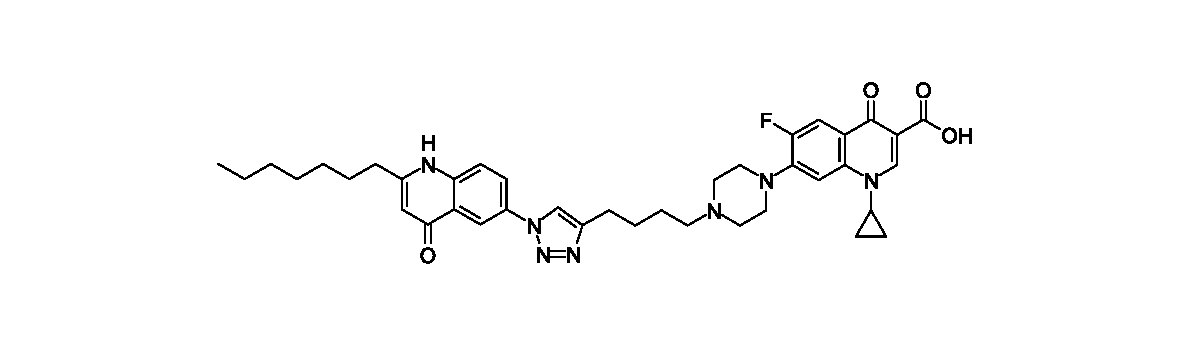
\includegraphics[scale=1]{6HHQT4Cip}
		\end{center}
	\end{scheme}
	
%LMO-2-006

50 \% water/\textit{t}-BuOH (1 ml) was degassed by bubbling \ce{N2} through it. This was then added to a mixture of 1-cyclopropyl-6-fluoro-7-(4-(hex-5-yn-1-yl)piperazin-1-yl)-4-oxo-1,4\hyp{}dihydro\-quinoline-3-carboxylic acid \compound{cmpd:Y4Cip} (4.1 mg, 10.0 $\mu$mol, 1 eq.) and 6-azido-2-heptylquinolin-4(1\textit{H})-one \compound{cmpd:azHHQ} (2.8 mg, 10.0 $\mu$mol, 1 eq.).
A similarly degassed solution of \ce{CuSO4.5H2O} (125 $\mu$g, 0.5 $\mu$mol, 0.05 eq. 50 mM), THPTA (218 $\mu$g, 0.5 $\mu$mol, 0.05 eq. 50 mM) and sodium ascorbate (198 $\mu$g, 1 $\mu$mol, 0.1 eq., 100 mM) in 50 \% water/\textit{t}-BuOH (10 $\mu$l) was then added. 
The mixture was stirred at r.t. under argon for 1.5 h, then the reaction mixture was evaporated under reduced pressure. The residue was purified by preparative HPLC (50-100 \% acetonitrile/water over 20 min).
The combined pure fractions were evaporated under reduced pressure and then partitioned between \ce{NaHCO3} (aq., sat., 10 ml) and 10 \% \textit{i}-PrOH/\ce{CHCl3} (10 ml). The organic layer was dried with \ce{MgSO4} and evaporated under reduced pressure.
\compound{cmpd:6HHQT4Cip} was obtained as a white amorphous solid (8.6 mg, 2.7 $\mu$mol, 27.0 \%). %rough
\\[1\baselineskip]
%\noindent{\textbf{TLC} \textit{R$_f$} = ?? (??)}
%\\[1\baselineskip]
%\noindent{\textbf{mp} \textit{T} / $^{\circ}$C = ?? (??)}
%\\[1\baselineskip]
\noindent{\textbf{IR} (neat) $\nu_{max}$ / cm$^{-1}$ = 
	%2980.4
	%2934.0
	%1607.7
	%1597.3	
	2927.0 (C-H),
	2865.5 (C-H),
	1715.5 (carboxylic acid C=O),
	%1672.5 \todo{is this TFA? redo}
	1631.0 (ciprofloxacin quinolone C=O and HHQ C=O)}
\\[1\baselineskip]
\noindent{\textbf{$^{1}$H NMR} (500 MHz, DMSO d$_6$)
	15.12 (br s, 1 H, \underline{C}(=O)OH), 
	11.79 (s, 1 H, N\underline{H}), 
	8.75 (s, 1 H, NC\underline{H}=CCH$_2$), 
	8.71 (s, 1 H, \textit{ortho} to C(=O)OH), 
	8.40 (d, \textit{J} = 2.7 Hz, 1 H, \textit{ortho} to C(=O) and \textit{ortho} to N), 
	8.18 (dd, \textit{J} = 8.9, 2.6 Hz, 1 H, \textit{para} to C(=O) and \textit{ortho} to N), 
	7.99 (d, \textit{J} = 13.0 Hz, 1 H, \textit{ortho} to F), 
	7.75 (d, \textit{J} = 9.0 Hz, 1 H, \textit{meta} to C(=O) and \textit{meta} to N), 
	7.62 (d, \textit{J} = 7.8 Hz, 1 H, \textit{meta} to F), 
	6.02 (s, 1 H, NHC=C\underline{H}C(=O)), 
	3.85 (tt, \textit{J} = 7.0, 4.0 Hz, 1 H, NC\underline{H}(CH$_2$)$_2$), 
	3.23 - 3.30 (m, 10 H, C\underline{H}$_2$N(C\underline{H}$_2$C\underline{H}$_2$)C\underline{H}$_2$C\underline{H}$_2$), 
	2.82 (t, \textit{J} = 5.9 Hz, 2 H, NCH=CC\underline{H}$_2$), 
	2.63 (t, \textit{J} = 7.9 Hz, 2 H, C\underline{H}$_2$C=CHC(=O)), 
	1.76 - 1.81 (m, 4 H, NCH=CCH$_2$C\underline{H}$_2$C\underline{H}$_2$), 
	1.70 (quin, \textit{J} = 7.2 Hz, 2 H, C\underline{H}$_2$CH$_2$C=CHC(=O)), 
	1.15 - 1.38 (m, 12 H, CH$_3$C\underline{H}$_2$C\underline{H}$_2$C\underline{H}$_2$C\underline{H}$_2$, NCH(C\underline{H}H)$_2$ and NCH(CH\underline{H})$_2$), 
	0.87 (t, \textit{J} = 6.9 Hz, 3 H, C\underline{H}$_3$)}
\\[1\baselineskip]
\noindent{\textbf{$^{13}$C NMR} (126 MHz, DMSO d$_6$) $\delta$ / ppm = 
	176.4 (\underline{C}(=O)CC(=O)OH), 
	176.3 (CH\underline{C}(=O)), 
	165.8 (\underline{C}(=O)OH), 
	154.3 (CCH\underline{C}(=O)), 
	152.9 (d, \textit{J} = 240.1 Hz, \textit{ipso} to F), 
	148.3 (\underline{C}H=CC(=O)OH), 
	147.5 (NCH\underline{C}CH$_2$), 
	143.3 (d, \textit{J} = 8.5 Hz, \textit{ortho} to F and \textit{ipso} to N), 
	139.6 (\textit{ipso} to NH), 
	139.0 (\textit{para} to F), 
	132.0 (\textit{para} to NH), 
	124.9 (\textit{ipso} to C(=O) and \textit{ortho} to NH), 
	123.6 (\textit{para} to C(=O) and \textit{meta} to NH), 
	120.5 (N\underline{C}H=CCH$_2$), 
	120.0 (\textit{meta} to C(=O) and \textit{meta} to N), 
	119.6 (d, \textit{J} = 9.6 Hz, \textit{ipso} to C(=O) and \textit{para} to N), 
	115.1 (\textit{ortho} to C(=O) and \textit{ortho} to N), 
	111.3 (d, \textit{J} = 28.8 Hz, \textit{ortho} to F and \textit{ortho} to C(=O)), 
	107.9 (\textit{meta} to F and \textit{meta} to C(=O)), 
	107.2 (\underline{C}HC(=O)), 
	106.9 (\underline{C}C(=O)OH), 
	55.4 (CH=CCH$_2$CH$_2$CH$_2$\underline{C}H$_2$N), 
	50.6 (CH$_2$CH$_2$CH$_2$N(\underline{C}H$_2$)\underline{C}H$_2$),
	46.5 (CH$_2$CH$_2$CH$_2$N(CH$_2$\underline{C}H$_2$)CH$_2$CH$_2$), 
	46.5 (CH$_2$CH$_2$CH$_2$N(CH$_2$CH$_2$)CH$_2$\underline{C}H$_2$),  
	36.0 (N\underline{C}H(CH$_2$)$_2$), 
	33.2 (\underline{C}H$_2$CNH), 
	31.2 (CH$_3$CH$_2$\underline{C}H$_2$), 
	28.3 - 28.5 (CH$_3$CH$_2$CH$_2$\underline{C}H$_2$\underline{C}H$_2$\underline{C}H$_2$), 
	25.6 (CH=CCH$_2$\underline{C}H$_2$), 
	24.4 (CH=C\allowbreak \underline{C}H$_2$), 
	22.7 (CH=CCH$_2$CH$_2$\underline{C}H$_2$), 
	22.0 (CH$_3$\underline{C}H$_2$), 
	13.9 (\underline{C}H$_3$), 
	7.6 (NCH(\underline{C}H$_2$)$_2$)}
\\[1\baselineskip]
%\noindent{\textbf{$^{19}$F NMR} (376.45 MHz, MeOD) $\delta$ / ppm = ??}%todo
%\\[1\baselineskip]
\noindent{\textbf{HRMS} (ESI$^+$) \textit{m}/\textit{z} / Da = 696.3667, [M+H]$^+$ found, [\ce{C39H47FN7O4}]$^+$ requires 696.3668}
\\[1\baselineskip]
The compound has not been reported previously.
	
	
\subsection{(\textit{S})-4-(4-(4-(4-((2,4-Diaminopyrimidin-5-yl)methyl)-2,6-dimethoxyphenoxy)\hfill\allowbreak butyl)-1\textit{H}-1,2,3-triazol-1-yl)-\textit{N}-(2-oxotetrahydrofuran-3-yl)butanamide \compound{cmpd:HL4T4Tri}}

	
%LMO-1-090 not pure, hydrolysis of the lactone and/or amide
%But was tested anyway??

	
\begin{scheme}[H]
	\begin{center}
		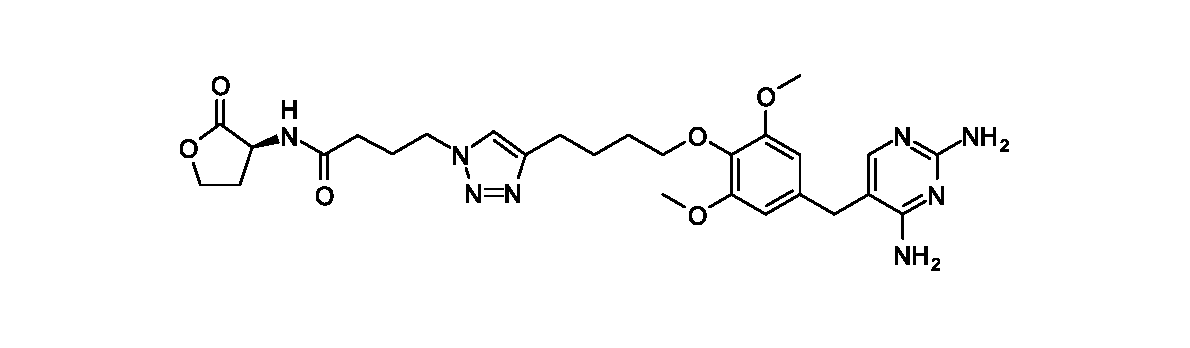
\includegraphics[scale=1]{HL4T4Tri}
	\end{center}
\end{scheme}
50 \% water/\textit{t}-BuOH (2 ml) was degassed by bubbling \ce{N2} through it. This was then added to a mixture of 5-(4-(hex-5-yn-1-yloxy)-3,5-dimethoxybenzyl)pyrimidine-2,4-diamine \compound{cmpd:Y4Tri} (20.6 mg, 50.0 $\mu$mol, 1 eq.) and (\textit{S})-4-azido-\textit{N}-(2-oxotetrahydrofuran-3-yl)butanamide \compound{cmpd:HL4N3} (15.9 mg, 75.0 $\mu$mol, 1.5 eq.).
Similarly degassed solutions of \ce{CuSO4.5H2O} (624 $\mu$g, 2.5 $\mu$mol, 0.05 eq. 50 mM), THPTA (1.09 mg, 2.5 $\mu$mol, 0.05 eq. 50 mM) and sodium ascorbate (991 $\mu$g, 5 $\mu$mol, 0.1 eq., 100 mM) in water (50 $\mu$l) were then added. An extra portion of \compound{cmpd:HL4N3} (10.6 mg, 50.0 $\mu$mol, 1 eq.) was added after 4 d. Extra portions of the catalysts were added after 9 d. 
After 2 weeks, the reaction mixture was extracted with \ce{CH2Cl2} (6$\times$10 ml) then dry-loaded onto \ce{SiO2} and purified by column chromatography using a Combiflash (\ce{SiO2}, 0-20 \% MeOH/\ce{CH2Cl2}).%guess
The combined pure fractions were dried with \ce{MgSO4} and evaporated under reduced pressure.
\compound{cmpd:HL4T4Tri} was obtained as a pale brown gum (4.8 mg, 8.4 $\mu$mol, 16.8 \%).
\\[1\baselineskip]
\noindent{\textbf{TLC} \textit{R$_f$} = 0.30 (30 \% MeOH/\ce{CH2Cl2})}
\\[1\baselineskip]
%\noindent{\textbf{mp} \textit{T} / $^{\circ}$C = ?? (??)}
%\\[1\baselineskip]
\noindent{\textbf{IR} (neat) $\nu_{max}$ / cm$^{-1}$ = 
	3340.5 (N-H),
	3303.3 (N-H),
	3182.5 (N-H),
	2933.8 (C-H),
	1774.2 (lactone C=O),
	1659.7 (amide C=O and pyrimidine)}
\\[1\baselineskip]
\noindent{\textbf{$^{1}$H NMR} (500 MHz, DMSO d$_6$) $\delta$ / ppm = 
	8.43 (d, \textit{J} = 8.0 Hz, 1 H, N\underline{H}), 
	7.80 (s, 1 H, NC\underline{H}=CCH$_2$), 
	7.46 (s, 1 H, C\underline{H}N=CNH$_2$), 
	6.68 (br s, 2 H, CH$_2$CCN\underline{H}$_2$), 
	6.53 (s, 2 H, \textit{meta} to CH$_2$), 
	6.21 (br s, 2 H, CHN=CN\underline{H}$_2$), 
	4.49 (dt, \textit{J} = 10.7, 8.6 Hz, 1 H, C\underline{H}NH), 
	4.32 (td, \textit{J} = 8.7, 1.6 Hz, 1 H, C\underline{H}HOC(=O)), 
	4.29 (t, \textit{J} = 6.8 Hz, 2 H, C\underline{H}$_2$N), 
	4.19 (ddd, \textit{J} = 10.6, 8.7, 6.5 Hz, 1 H, CH\underline{H}OC(=O)), 
	3.79 (t, \textit{J} = 6.2 Hz, 2 H, CH$_2$CH$_2$C\underline{H}$_2$O), 
	3.68 (s, 6 H, C\underline{H}$_3$), 
	3.53 (br s, 2 H, CC\underline{H}$_2$C), 
	2.63 (t, \textit{J} = 7.5 Hz, 2 H, CH=CC\underline{H}$_2$), 
	2.37 (dddd, \textit{J} = 12.2, 8.9, 6.7, 1.8 Hz, 1 H, C\underline{H}HCHNH), 
	2.08 - 2.15 (m, 3 H, CH\underline{H}CHNH and C(=O)C\underline{H}$_2$), 
	2.00 (quin, \textit{J} = 7.2 Hz, 2 H, C\underline{H}$_2$CH$_2$N), 
	1.72 (quin, \textit{J} = 7.3 Hz, 2 H, CH=CCH$_2$C\underline{H}$_2$), 
	1.61 (quin, \textit{J} = 6.7 Hz, 2 H, C\underline{H}$_2$CH$_2$O)}
\\[1\baselineskip]
\noindent{\textbf{$^{13}$C NMR} (126 MHz, DMSO d$_6$) $\delta$ / ppm = 
	175.8 (O\underline{C}=O), 
	171.9 (NH\underline{C}=O), 
	163.1 (C\underline{C}(NH$_2$)N), 
	159.7 (br s, N\underline{C}(NH$_2$)N), 
	153.2 (\textit{ipso} to OCH$_3$), 
	150.5 (br s, \underline{C}HNC(NH$_2$)N), 
	147.3 (NCH=\underline{C}CH$_2$CH$_2$), 
	135.2 (\textit{para} to CH$_2$O), 
	135.0 (\textit{ipso} to CH$_2$O), 
	122.1 (\underline{C}H=CCH$_2$CH$_2$), 
	107.3 (CH$_2$\underline{C}C(NH$_2$)=N), 
	106.2 (\textit{meta} to CH$_2$O), 
	72.3 (CH$_2$CH$_2$\underline{C}H$_2$O), 
	65.7 (O\underline{C}H$_2$CH$_2$CHNH), 
	56.2 (O\underline{C}H$_3$), 
	48.9 (\underline{C}H$_2$N), 
	48.3 (\underline{C}HNH), 
	32.9 (C\underline{C}H$_2$C), 
	32.0 (C(=O)\underline{C}H$_2$), 
	29.3 (CH$_2$\underline{C}H$_2$CH$_2$O), 
	28.4 (OCH$_2$\underline{C}H$_2$CHNH), 
	26.0 (\underline{C}H$_2$CH$_2$N), 
	25.7 (CH=CCH$_2$\underline{C}H$_2$), 
	24.9 (CH=C\underline{C}H$_2$CH$_2$)}
\\[1\baselineskip]
\noindent{\textbf{HRMS} (ESI$^+$) \textit{m}/\textit{z} / Da = 569.2834, [M+H]$^+$ found, [\ce{C27H37N8O6}]$^+$ requires 569.2836}
\\[1\baselineskip]
\noindent{[\bm{$\alpha$}]$_D^{20}$ / $^{\circ}$10$^{-1}$cm$^2$g$^{-1}$ = -4.6 (\textit{c} / g(100 ml)$^{-1}$ = 0.0433 , MeOH)}
\\[1\baselineskip]
The compound has not been reported previously.
	
\subsection{(\textit{S})-6-(4-(4-(4-((2,4-Diaminopyrimidin-5-yl)methyl)-2,6-dimethoxyphenoxy)\hfill\allowbreak butyl)-1\textit{H}-1,2,3-triazol-1-yl)-\textit{N}-(2-oxotetrahydrofuran-3-yl)hexanamide \compound{cmpd:HL6T4Tri}}

\begin{scheme}[H]
	\begin{center}
		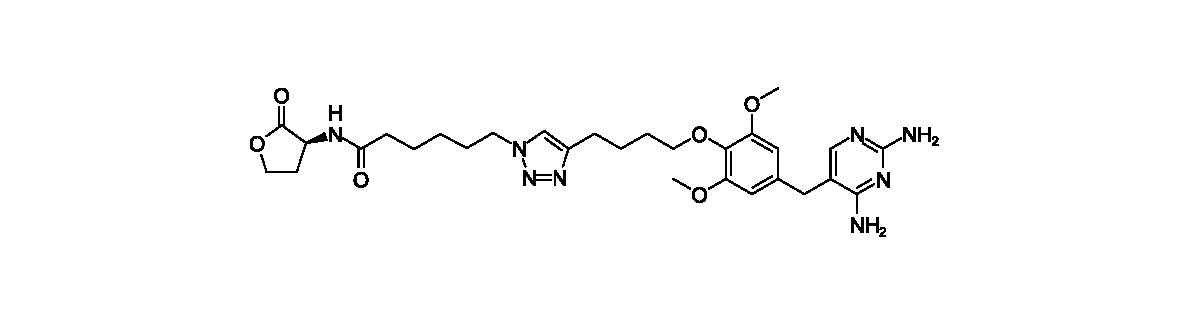
\includegraphics[scale=1]{HL6T4Tri}
	\end{center}
\end{scheme}

%LMO-1-090 (one of several with this number)

50 \% water/\textit{t}-BuOH (2 ml) was degassed by bubbling \ce{N2} through it. This was then added to a mixture of 5-(4-(hex-5-yn-1-yloxy)-3,5-dimethoxybenzyl)pyrimidine-2,4-diamine \compound{cmpd:Y4Tri} (20.6 mg, 50.0 $\mu$mol, 1 eq.) and (\textit{S})-6-azido-\textit{N}-(2-oxotetrahydrofuran-3-yl)hexanamide \compound{cmpd:HL6N3} (18.0 mg, 75.0 $\mu$mol, 1.5 eq.).
Similarly degassed solutions of \ce{CuSO4.5H2O} (624 $\mu$g, 2.5 $\mu$mol, 0.05 eq. 50 mM), THPTA (1.09 mg, 2.5 $\mu$mol, 0.05 eq. 50 mM) and sodium ascorbate (991 $\mu$g, 5 $\mu$mol, 0.1 eq., 100 mM) in water (50 $\mu$l) were then added. An extra portion of \compound{cmpd:HL6N3} (12.0 mg, 50.0 $\mu$mol, 1 eq.) was added after 4 d. Extra portions of the catalysts were added after 9 d. After 2 weeks the reaction mixture was extracted with \ce{CH2Cl2} (6$\times$10 ml) then dry-loaded onto \ce{SiO2} and purified by column chromatography using a Combiflash (\ce{SiO2}, 0-20 \% MeOH/\ce{CH2Cl2}). %guess
The combined pure fractions were dried with \ce{MgSO4} and evaporated under reduced pressure.
\compound{cmpd:HL6T4Tri} was obtained as a clear gum (8.0 mg, 13.4 $\mu$mol, 26.8 \%).
\\[1\baselineskip]
\noindent{\textbf{TLC} \textit{R$_f$} = 0.35 (30 \% MeOH/\ce{CH2Cl2})}
\\[1\baselineskip]
%\noindent{\textbf{mp} \textit{T} / $^{\circ}$C = ?? (??)}
%\\[1\baselineskip]
\noindent{\textbf{IR} (neat) $\nu_{max}$ / cm$^{-1}$ = 
	3336.0 (N-H),
	3208.7 (N-H),
	2941.1 (C-H),
	2869.2 (C-H),
	1775.2 (lactone C=O),
	1657.3 (amide C=O and pyrimidine)}
\\[1\baselineskip]
\noindent{\textbf{$^{1}$H NMR} (500 MHz, DMSO d$_6$) $\delta$ / ppm = 
	8.34 (d, \textit{J} = 8.0 Hz, 1 H, N\underline{H}), 
	7.83 (s, 1 H, NC\underline{H}=CCH$_2$), 
	7.50 (s, 1 H, C\underline{H}N=CNH$_2$), 
	6.54 (s, 2 H, \textit{meta} to CH$_2$), 
	6.17 (br s, 2 H, CH$_2$CCN\underline{H}$_2$), 
	5.77 (br s, 2 H, CHN=CN\underline{H}$_2$), 
	4.51 (ddd, \textit{J} = 11.0, 9.0, 8.1 Hz, 1 H, C\underline{H}NH), 
	4.33 (td, \textit{J} = 8.8, 1.9 Hz, 1 H, C\underline{H}HOC(=O)), 
	4.27 (t, \textit{J} = 7.1 Hz, 2 H, C\underline{H}$_2$N), 
	4.19 (ddd, \textit{J} = 10.5, 8.7, 6.5 Hz, 1 H, CH\underline{H}OC(=O)), 
	3.80 (t, \textit{J} = 6.3 Hz, 2 H, CH$_2$CH$_2$C\underline{H}$_2$O), 
	3.70 (s, 6 H, C\underline{H}$_3$), 
	3.52 (s, 2 H, CC\underline{H}$_2$C),  
	2.64 (t, \textit{J} = 7.5 Hz, 2 H, CH=CC\underline{H}$_2$), 
	2.36 (dddd, \textit{J} = 12.1, 8.9, 6.7, 1.8 Hz, 1 H, C\underline{H}HCHNH), 
	2.06 - 2.16 (m, 3 H, CH\underline{H}CHNH and C(=O)C\underline{H}$_2$), 
	1.78 (quin, \textit{J} = 7.4 Hz, 2 H, C\underline{H}$_2$CH$_2$N), 
	1.73 (quin, \textit{J} = 7.7 Hz, 2 H, CH=CCH$_2$C\underline{H}$_2$), 
	1.63 (quin, \textit{J} = 6.8 Hz, 2 H, C\underline{H}$_2$CH$_2$O), 
	1.52 (quin, \textit{J} = 7.5 Hz, 2 H, C(=O)CH$_2$C\underline{H}$_2$), 
	1.17 - 1.27 (m, 2 H, C(=O)CH$_2$CH$_2$C\underline{H}$_2$)}
\\[1\baselineskip]
\noindent{\textbf{$^{13}$C NMR} (125 MHz, DMSO d$_6$) $\delta$ / ppm = 
	175.4 (O\underline{C}=O), 
	172.0 (NH\underline{C}=O), 
	162.2 (C\underline{C}(NH$_2$)N), 
	161.8 (N\underline{C}(NH$_2$)N), 
	154.8 (\underline{C}HNC(NH$_2$)N), 
	152.8 (\textit{ipso} to OCH$_3$), 
	146.7 (CH=\underline{C}CH$_2$CH$_2$), 
	135.5 (\textit{para} to CH$_2$O), 
	134.8 (\textit{ipso} to CH$_2$O), 
	121.6 (\underline{C}H=CCH$_2$CH$_2$), 
	105.9 (CH$_2$\underline{C}C(NH$_2$)=N), 
	105.8 (\textit{meta} to CH$_2$O), 
	71.9 (CH$_2$CH$_2$\allowbreak \underline{C}H$_2$O), 
	65.2 (O\underline{C}H$_2$CH$_2$CHNH), 
	55.8 (O\underline{C}H$_3$), 
	49.0 (\underline{C}H$_2$N), 
	47.8 (\underline{C}HNH), 
	34.8 (C(=O)\underline{C}H$_2$), 
	32.9 (C\underline{C}H$_2$C), 
	29.4 (\underline{C}H$_2$CH$_2$N), 
	29.1 (CH$_2$\underline{C}H$_2$CH$_2$O), 
	28.2 (OCH$_2$\underline{C}H$_2$CHNH), 
	25.5 (CH=CCH$_2$\underline{C}H$_2$), 
	25.3 (C(=O)CH$_2$CH$_2$\allowbreak \underline{C}H$_2$), 
	24.7 (CH=C\underline{C}H$_2$CH$_2$), 
	24.4 (C(=O)CH$_2$\underline{C}H$_2$)}
\\[1\baselineskip]
\noindent{\textbf{HRMS} (ESI$^+$) \textit{m}/\textit{z} / Da = 597.3149, [M+H]$^+$ found, [\ce{C29H41N8O6}]$^+$ requires 597.3144}
\\[1\baselineskip]
\noindent{[\bm{$\alpha$}]$_D^{20}$ / $^{\circ}$10$^{-1}$cm$^2$g$^{-1}$ = -3.6 (\textit{c} / g(100 ml)$^{-1}$ = 0.11 , MeOH)}
\\[1\baselineskip]
The compound has not been reported previously.

\subsection{6-(4-(4-(4-((2,4-Diaminopyrimidin-5-yl)methyl)-2,6-dimethoxyphenoxy)but\allowbreak y\allowbreak l)\hyp{}1\textit{H}-1,2,3-triazol-1-yl)-2-heptylquinolin-4(1\textit{H})-one \compound{cmpd:6HHQT4Tri}}
	
	\begin{scheme}[H]
		\begin{center}
			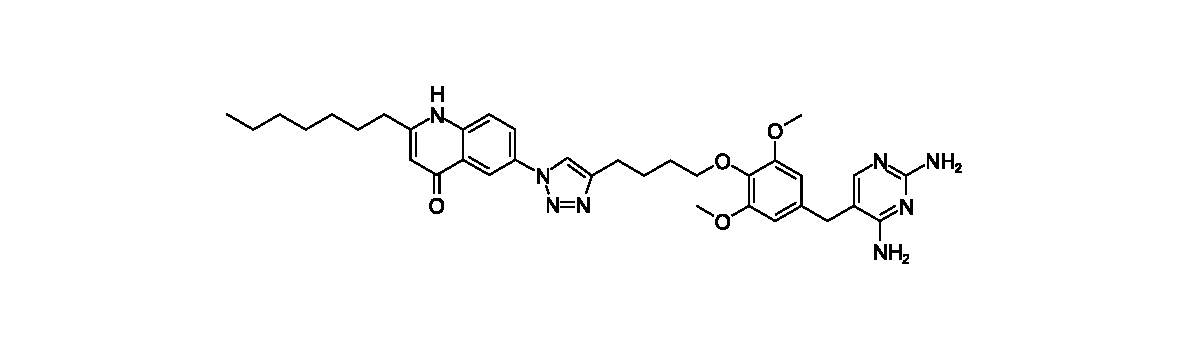
\includegraphics[scale=1]{6HHQT4Tri}
		\end{center}
	\end{scheme}
	
%LMO-2-003 and 005?

50 \% water/\textit{t}-BuOH (1 ml) was degassed by bubbling \ce{N2} through it. This was then added to a mixture of 5-(4-(hex-5-yn-1-yloxy)-3,5-dimethoxybenzyl)pyrimidine-2,4-diamine \compound{cmpd:Y4Tri} (3.6 mg, 10.0 $\mu$mol, 1 eq.) and 6-azido-2-heptylquinolin-4(1\textit{H})-one \compound{cmpd:azHHQ} (2.8 mg, 10.0 $\mu$mol, 1 eq.).
A similarly degassed solution of 
\ce{CuSO4.5H2O} (125 $\mu$g, 0.5 $\mu$mol, 0.05 eq. 50 mM), 
THPTA (218 $\mu$g, 0.5 $\mu$mol, 0.05 eq. 50 mM) and 
sodium ascorbate (198 $\mu$g, 1 $\mu$mol, 0.1 eq., 100 mM) in water (10 $\mu$l) was then added. 
The mixture was stirred at r.t. under argon for 1.5 h, then evaporated under reduced pressure. The residue was purified by preparative HPLC (5-100 \% acetonitrile/water over 20 min).
The combined pure fractions were evaporated under reduced pressure and then partitioned between \ce{NaHCO3} (aq., sat., 10 ml) and 10 \% \textit{i}-PrOH/\ce{CHCl3} (10 ml). The organic layer was dried with \ce{MgSO4} and evaporated under reduced pressure.
\compound{cmpd:6HHQT4Tri} was obtained as a clear gum (2.6 mg, 4.1 $\mu$mol, 41.0 \%).
\\[1\baselineskip]
\noindent{\textbf{TLC} \textit{R$_f$} = 0.17 (20 \% MeOH/\ce{CH2Cl2)}}
\\[1\baselineskip]
%\noindent{\textbf{mp} \textit{T} / $^{\circ}$C = ?? (??)}
%\\[1\baselineskip]
\noindent{\textbf{IR} (neat) $\nu_{max}$ / cm$^{-1}$ = 
	2927.7 (C-H),
	2855.5 (C-H),
	1664.1 (pyrimidine),
	1645.4 (pyrimidine and HHQ C=O)}
\\[1\baselineskip]
\noindent{\textbf{$^{1}$H NMR} (500 MHz, DMSO d$_6$) $\delta$ / ppm = 
	11.80 (s, 1 H, N\underline{H}), 
	8.69 (s, 1 H, NC\underline{H}=CCH$_2$), 
	8.41 (d, \textit{J} = 2.7 Hz, 1 H, \textit{ortho} to C=O), 
	8.17 (dd, \textit{J} = 9.0, 2.6 Hz, 1 H, \textit{para} to C=O), 
	7.73 (d, \textit{J} = 9.0 Hz, 1 H, \underline{ortho} to NH), 
	7.51 (br s, 4 H, NH$_2$), 
	7.41 (s, 1 H, C\underline{H}N=CNH$_2$), 
	6.61 (s, 2 H, \textit{meta} to CH$_2$), 
	6.02 (d, \textit{J} = 1.8 Hz, 1 H, C(=O)C\underline{H}), 
	3.86 (t, \textit{J} = 6.3 Hz, 2 H, C\underline{H}$_2$O), 
	3.73 (s, 6 H, OC\underline{H}$_3$), 
	3.57 - 3.62 (m, 2 H, CC\underline{H}$_2$C), 
	2.78 (t, \textit{J} = 7.5 Hz, 2 H, CH=CC\underline{H}$_2$), 
	2.63 (t, \textit{J} = 7.3 Hz, 2 H, HNCC\underline{H}$_2$), 
	1.85 (quin, \textit{J} = 7.5 Hz, 2 H, CH=CCH$_2$C\underline{H}$_2$), 
	1.61 - 1.78 (m, 4 H, HNCCH$_2$C\underline{H}$_2$ and CH=CCH$_2$CH$_2$C\underline{H}$_2$), 
	1.31 - 1.40 (m, 4 H, HNCCH$_2$CH$_2$C\underline{H}$_2$C\underline{H}$_2$), 
	1.25 - 1.31 (m, 4 H, CH$_3$C\underline{H}$_2$C\underline{H}$_2$), 
	0.86 (t, \textit{J} = 7.2 Hz, 3 H, C\underline{H}$_3$CH$_2$)}
\\[1\baselineskip]
\noindent{\textbf{$^{13}$C NMR} (125 MHz, DMSO d$_6$) $\delta$ / ppm = 
	176.4 (\underline{C}=O), 
	164.1 (C\underline{C}(NH$_2$)N), 
	154.3 (HN\underline{C}), 
	154.2 (N\underline{C}(NH$_2$)N), 
	153.1 (\textit{ipso} to OCH$_3$), 
	148.3 (CH=\underline{C}CH$_2$CH$_2$), 
	140.2 (\underline{C}HNC(NH$_2$)N), 
	139.6 (\textit{ipso} to NH), 
	135.4 (\textit{ipso} to CH$_2$O), 
	132.8 (\textit{para} to CH$_2$O), 
	132.1 (\textit{para} to NH), 
	124.9 (\textit{ipso} to C=O), 
	123.7 (\textit{para} to C=O), 
	120.3 (\underline{C}H=CCH$_2$CH$_2$), 
	120.0 (\textit{meta} to C=O and \textit{ortho} to NH), 
	115.1 (\textit{ortho} to C=O and \textit{meta} to NH), 
	109.0 (CH$_2$\underline{C}C(NH$_2$)=N), 
	108.0 (C(=O)\underline{C}H), 
	106.3 (\textit{meta} to CH$_2$O), 
	72.0 (CH$_2$CH$_2$\underline{C}H$_2$O), 
	56.0 (O\underline{C}H$_3$), 
	33.3 (HNC\underline{C}H$_2$), 
	32.1 (C\underline{C}H$_2$C), 
	31.2 (CH$_3$CH$_2$\underline{C}H$_2$), 
	29.1 (\underline{C}H$_2$CH$_2$O), 
	28.3 - 28.6 (CH$_3$CH$_2$CH$_2$\underline{C}H$_2$\underline{C}H$_2$\underline{C}H$_2$), 
	25.3 (\underline{C}H$_2$CH$_2$CH$_2$O), 
	24.7 (CH=C\underline{C}H$_2$), 
	22.1 (CH$_3$\underline{C}H$_2$), 
	14.0 (\underline{C}H$_3$CH$_2$)}
\\[1\baselineskip]
\noindent{\textbf{HRMS} (ESI$^+$) \textit{m}/\textit{z} / Da = 641.3557, [M+H]$^+$ found, [\ce{C35H45N8O4}]$^+$ 641.3558}
\\[1\baselineskip]
The compound has not been reported previously.

\subsection{2-(6-(4-(4-(4-((2,4-Diaminopyrimidin-5-yl)methyl)-2,6-dimethoxyphenoxy)\allowbreak bu\allowbreak tyl)-1\textit{H}-1,2,3-triazol-1-yl)hexyl)-3-hydroxyquinolin-4(1\textit{H})-one \compound{cmpd:PQST4Tri}}
	
	\begin{scheme}[H]
		\begin{center}
			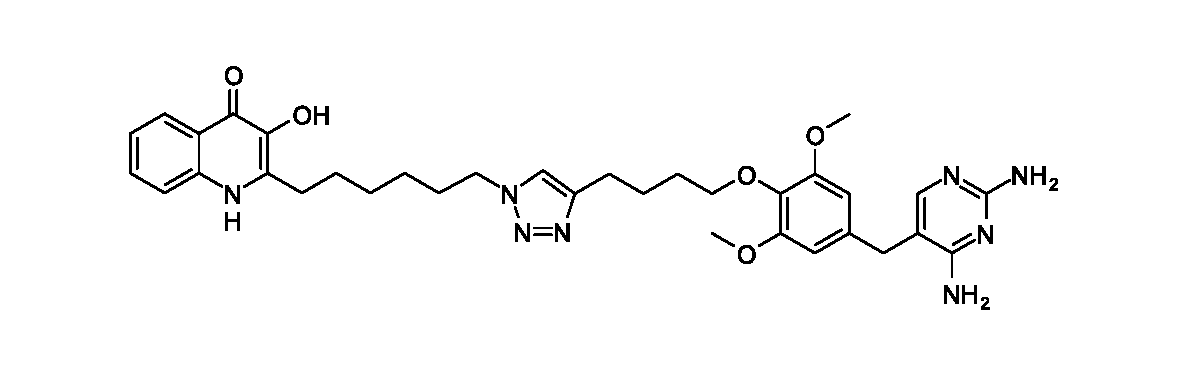
\includegraphics[scale=1]{PQST4Tri}
		\end{center}
	\end{scheme}
	
%LMO-2-002

50 \% water/\textit{t}-BuOH (1 ml) was degassed by bubbling \ce{N2} through it. This was then added to a mixture of 5-(4-(hex-5-yn-1-yloxy)-3,5-dimethoxybenzyl)pyrimidine-2,4-diamine \compound{cmpd:Y4Tri} (14.2 mg, 39.8 $\mu$mol, 1 eq.) and 2-(6-azidohexyl)-3-hydroxyquinolin-4(1H)-one \compound{cmpd:PQSaz} (11.4 mg, 39.8 $\mu$mol, 1 eq.).
A similarly degassed solution of 
\ce{CuSO4.5H2O} (1.25 mg, 5 $\mu$mol, 0.125 eq. 50 mM), 
THPTA (2.18 mg, 5 $\mu$mol, 0.125 eq. 50 mM) and 
sodium ascorbate (1.98 mg, 10 $\mu$mol, 0.25 eq., 100 mM) in water (100 $\mu$l) was then added.
The mixture was stirred at r.t. under argon for 3 h, then MeOH (1 ml) was added and the reaction mixture was dry-loaded onto \ce{SiO2} and purified by column chromatography (\ce{SiO2}, 0-20 \% MeOH/\ce{CH2Cl2}).
The combined pure fractions were dried with \ce{MgSO4} and evaporated under reduced pressure. 
\compound{cmpd:PQST4Tri} was obtained as a pale brown amorphous solid (4.7 mg, 7.3 $\mu$mol, 18.3 \%).
\\[1\baselineskip]
\noindent{\textbf{TLC} \textit{R$_f$} = 0.21 (20 \% MeOH/\ce{CH2Cl2})}
\\[1\baselineskip]
%\noindent{\textbf{mp} \textit{T} / $^{\circ}$C = ?? (??)}
%\\[1\baselineskip]
\noindent{\textbf{IR} (neat) $\nu_{max}$ / cm$^{-1}$ = 
	2924.8 (C-H),
	2853.4 (C-H),
	1660.0 (pyrimidine),
	1638.8 (pyrimidine and PQS C=O)}
\\[1\baselineskip]
\noindent{\textbf{$^{1}$H NMR} (500 MHz, DMSO d$_6$) $\delta$ / ppm = 
	11.53 (br s, 1 H, N\underline{H}), 
	8.09 (d, \textit{J} = 8.0 Hz, 1 H, \textit{ortho} to C=O), 
	7.83 (s, 1 H, NC\underline{H}=CCH$_2$), 
	7.48 - 7.57 (m, 3 H, \textit{para} to C=O, \textit{ortho} to NH and C\underline{H}N=CNH$_2$), 
	7.21 (ddd, \textit{J} = 8.0, 6.3, 1.5 Hz, 1 H, \textit{para} to NH), 
	6.55 (s, 2 H, \textit{meta} to CH$_2$), 
	4.28 (t, \textit{J} = 7.1 Hz, 2 H, C\underline{H}$_2$N), 
	3.80 (t, \textit{J} = 6.2 Hz, 2 H, C\underline{H}$_2$O), 
	3.70 (s, 6 H, C\underline{H}$_3$), 
	3.53 (d, \textit{J} = 0.3 Hz, 2 H, CC\underline{H}$_2$C), 
	2.73 (t, \textit{J} = 7.5 Hz, 2 H, HNCC\underline{H}$_2$), 
	2.64 (t, \textit{J} = 7.4 Hz, 2 H, CH=CC\underline{H}$_2$), 
	1.80 (quin, \textit{J} = 7.4 Hz, 2 H, C\underline{H}$_2$CH$_2$N), 
	1.73 (quin, \textit{J} = 7.5 Hz, 2 H, CH=CCH$_2$C\underline{H}$_2$), 
	1.66 (quin, \textit{J} = 7.2 Hz, 2 H, HNCCH$_2$C\underline{H}$_2$), 
	1.62 (quin, \textit{J} = 6.8 Hz, 2 H, C\underline{H}$_2$CH$_2$O), 
	1.33 - 1.40 (m, 2 H, HNCCH$_2$CH$_2$C\underline{H}$_2$), 
	1.27 - 1.32 (m, 2 H, HNCCH$_2$CH$_2$CH$_2$C\underline{H}$_2$)}
\\[1\baselineskip]
\noindent{\textbf{$^{13}$C NMR} (125 MHz, DMSO d$_6$) $\delta$ / ppm = 
	168.9 (\underline{C}=O), 
	162.5 (C\underline{C}(NH$_2$)N), 
	162.5 (N\underline{C}(NH$_2$)N), 
	152.9 (\underline{C}HNC(NH$_2$)N), 
	152.8 (\textit{ipso} to OCH$_3$), 
	146.8 (CH=\underline{C}CH$_2$CH$_2$), 
	137.7 (\underline{C}OH), 
	137.3 (\textit{para} to OH), 
	135.4 (HN\underline{C}), 
	135.1 (\textit{para} to CH$_2$O), 
	134.8 (\textit{ipso} to CH$_2$O), 
	129.9 (\textit{para} to C=O), 
	124.4 (\textit{ortho} to C=O and \textit{meta} to NH), 
	122.1 (\textit{ipso} to C=O), 
	121.5 (\textit{para} to NH), 
	121.4 (\underline{C}H=CCH$_2$CH$_2$), 
	117.7 (\textit{meta} to C=O and \textit{ortho} to NH), 
	106.2 (CH$_2$\underline{C}C(NH$_2$)=N), 
	105.8 (\textit{meta} to CH$_2$O), 
	71.9 (CH$_2$CH$_2$\underline{C}H$_2$O), 
	55.8 (O\underline{C}H$_3$), 
	49.0 (\underline{C}H$_2$N), 
	32.8 (C\underline{C}H$_2$C), 
	29.5 (\underline{C}H$_2$CH$_2$N), 
	29.0 (\underline{C}H$_2$CH$_2$O), 
	28.1 (HNCCH$_2$CH$_2$\underline{C}H$_2$), 
	27.9 (HNC\underline{C}H$_2$), 
	27.6 (HNCCH$_2$\underline{C}H$_2$), 
	25.6 (\underline{C}H$_2$CH$_2$CH$_2$N), 
	25.4 (\underline{C}H$_2$CH$_2$CH$_2$O), 
	24.6 (CH=C\underline{C}H$_2$CH$_2$)}
\\[1\baselineskip]
\noindent{\textbf{HRMS} (ESI$^+$) \textit{m}/\textit{z} / Da = 643.3365, [M+H]$^+$ found, [\ce{C34H43N8O5}]$^+$ requires 643.3351}
\\[1\baselineskip]
The compound has not been reported previously.







%\subsection{(\textit{S})-1-Cyclopropyl-6-fluoro-4-oxo-7-(4-(4-(1-(2-oxo-2-((2-oxotetrahydrofuran\hyp{}3-yl)amino)ethyl)-\textit{1H}-1,2,3-triazol-4-yl)butyl)piperazin-1-yl)-1,4-dihydroqui\hyp{}noline\hyp{}3-carboxylic acid \compound{cmpd:HL2N3hexpipcip}}
%
%%notmade
%
%\begin{scheme}[H]
%	\begin{center}
%		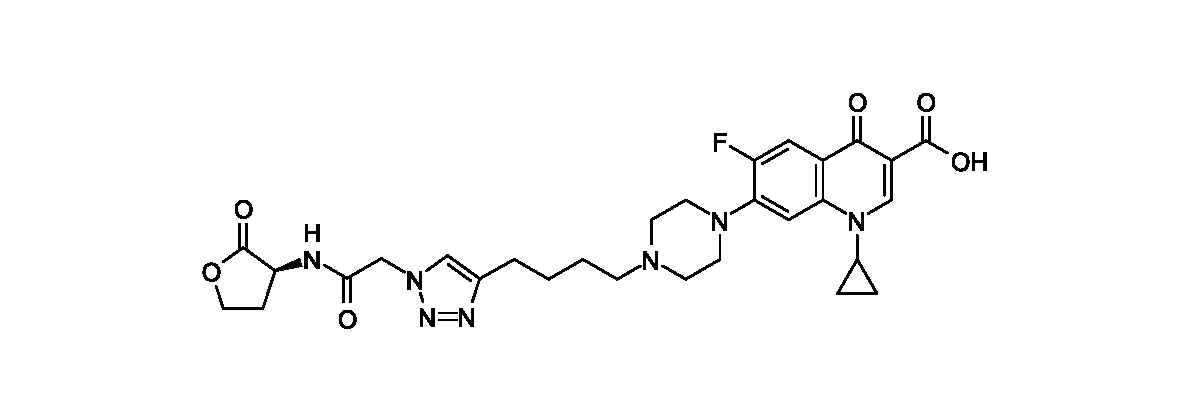
\includegraphics[scale=1]{HL2hexpipcip}
%	\end{center}
%\end{scheme}
%
%1-Cyclopropyl-6-fluoro-7-(4-(hex-5-yn-1-yl)piperazin-1-yl)-4-oxo-1,4\hyp{}dihydro\-quinoline-3-carboxylic acid \compound{cmpd:hexpipcip} (2 mg, 4.86 $\mu$mol, 1 eq.), (\textit{S})-2-azido-\textit{N}-(2-oxotetrahydrofuran-3-yl)acetamide \compound{cmpd:HL2N3} (0.9 mg, 4.89 $\mu$mol, 1 eq.) and \textit{t}-BuOH (0.1 ml) were placed under argon, followed by addition of \ce{CuSO4} (1 mM, aq., 48.6 $\mu$L, 48.6 nmol, 0.02 eq.) and sodium \textsc{l}-ascorbate (1 mM, aq., 243 $\mu$L, 243 nmol, 0.1 eq.). The mixture was stirred at $50\ ^{\circ}$C for 4 d, after which full consumption of \compound{cmpd:hexpipcip} and the appearance of a product with the correct \textit{m}/\textit{z} was seen.
%\\[1\baselineskip]
%\noindent{LR MS (ESI$^+$) \textit{m}/\textit{z} / Da = 596.4, [M+H]$^+$, [\ce{C29H35FN7O6}]$^+$, \textit{m}/\textit{z} / Da required = 596.2627}
%
%
%
%

%
%
%\subsection{(S)-1-cyclopropyl-6-fluoro-4-oxo-7-(4-(4-(1-(6-oxo-6-((2-oxotetrahydrofuran-3-yl)amino)hexyl)-1H-1,2,3-triazol-4-yl)butyl)piperazin-1-yl)-1,4-dihydroquinoline-3-carboxylic acid \compound{cmpd:HL6hexpipcip}}
%
%%notmade
%
%\begin{scheme}[H]
%	\begin{center}
%		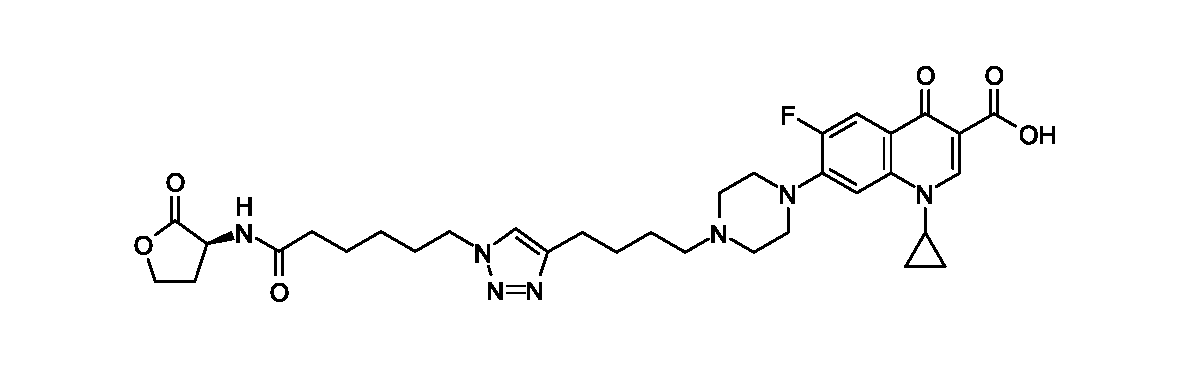
\includegraphics[scale=1]{HL6hexpipcip}
%	\end{center}
%\end{scheme}
%
%
%\subsection{1-cyclopropyl-6-fluoro-7-(4-(4-(1-(2-heptyl-4-oxo-1,4-dihydroquinolin-6-yl)-1H-1,2,3-triazol-4-yl)butyl)piperazin-1-yl)-4-oxo-1,4-dihydroquinoline-3-carboxylic acid \compound{cmpd:azHHQhexpipcip}}
%
%%notmade
%
%\begin{scheme}[H]
%	\begin{center}
%		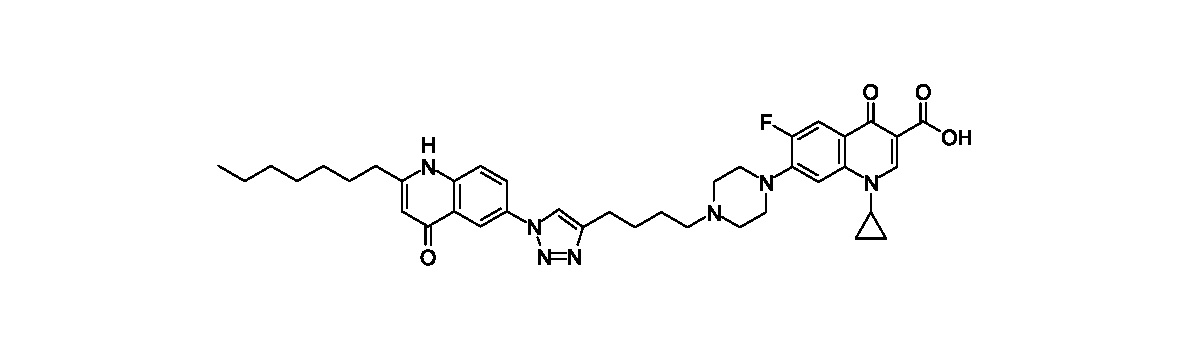
\includegraphics[scale=1]{azHHQhexpipcip}
%	\end{center}
%\end{scheme}
%
%\subsection{1-cyclopropyl-6-fluoro-7-(4-(4-(1-(2-heptyl-3-hydroxy-4-oxo-1,4-dihydroquinolin-6-yl)-1H-1,2,3-triazol-4-yl)butyl)piperazin-1-yl)-4-oxo-1,4-dihydroquinoline-3-carboxylic acid \compound{cmpd:azPQShexpipcip}}
%
%%notmade
%
%\begin{scheme}[H]
%	\begin{center}
%		%\includegraphics[scale=1]{azPQShexpipcip}
%	\end{center}
%\end{scheme}
%
%\subsection{1-cyclopropyl-6-fluoro-4-oxo-7-(4-(4-(1-(6-(4-oxo-1,4-dihydroquinolin-2-yl)hexyl)-1H-1,2,3-triazol-4-yl)butyl)piperazin-1-yl)-1,4-dihydroquinoline-3-carboxylic acid \compound{cmpd:HHQazhexpipcip}}
%
%%notmade
%
%\begin{scheme}[H]
%	\begin{center}
%		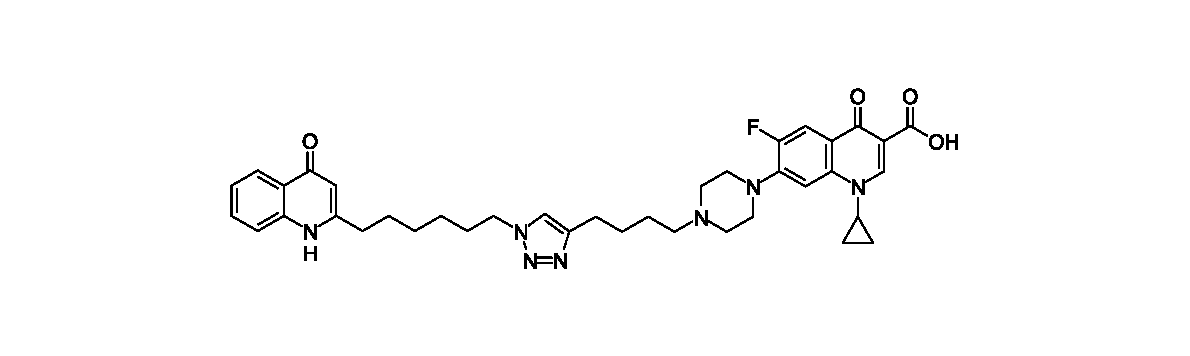
\includegraphics[scale=1]{HHQazhexpipcip}
%	\end{center}
%\end{scheme}
%
%\subsection{1-cyclopropyl-6-fluoro-7-(4-(4-(1-(6-(3-hydroxy-4-oxo-1,4-dihydroquinolin-2-yl)hexyl)-1H-1,2,3-triazol-4-yl)butyl)piperazin-1-yl)-4-oxo-1,4-dihydroquinoline-3-carboxylic acid \compound{cmpd:PQSazhexpipcip}}
%
%%notmade
%
%\begin{scheme}[H]
%	\begin{center}
%		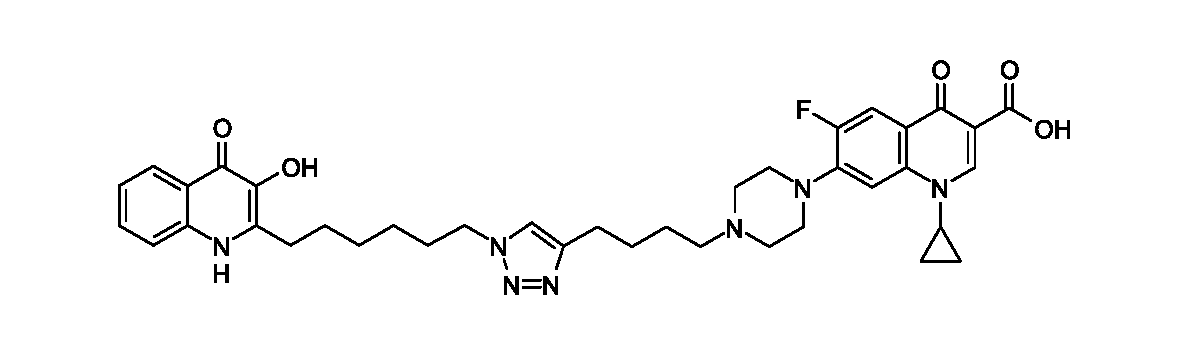
\includegraphics[scale=1]{PQSazhexpipcip}
%	\end{center}
%\end{scheme}
%
%\subsection{Methyl 7-(4-(4-(tert-butoxy)-4-oxobutyl)piperazin-1-yl)-1-cyclopropyl-6-fluoro-4-oxo-1,4-dihydroquinoline-3-carboxylate \compound{cmpd:tBu4CipMe}}
%
%%LMO-2-081
%
%\begin{scheme}[H]
%	\begin{center}
%		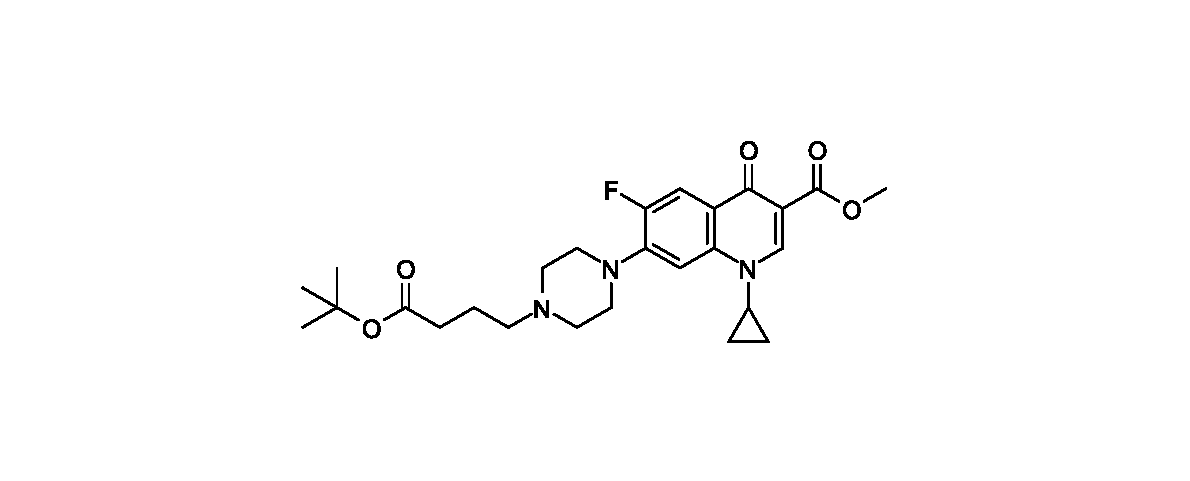
\includegraphics[scale=1]{tBu4CipMe}
%	\end{center}
%\end{scheme}
%
%Methyl 1-cyclopropyl-6-fluoro-4-oxo-7-(piperazin-1-yl)-1,4-dihydroquinoline-3-carboxylate \compound{cmpd:CipMe} (200 mg, ? mmol, 1 eq.), \textit{tert}-butyl 4-bromobutanoate ( 102 $\mu$l, ? mmol, ? eq.), sodium iodide
%\\[1\baselineskip]
%\noindent{$^{1}$H NMR (400 MHz, \ce{CDCl3}) $\delta$ / ppm = 
%	8.39 (s, 1 H, \textit{ortho} to C(=O)OH), 
%	7.82 (d, \textit{J} = 13.3 Hz, 1 H, \textit{ortho} to F), 
%	7.17 (d, \textit{J} = 7.2 Hz, 1 H, \textit{meta} to F), 
%	3.83 (s, 3 H, C\underline{H}$_3$),
%	3.40 (m, 1 H, NC\underline{H}(CH$_2$)$_2$),
%	3.22 (m, 4 H, CH$_2$N(C\underline{H}$_2$)C\underline{H}$_2$), 
%	2.63 (m, 4 H, CH$_2$N(CH$_2$C\underline{H}$_2$)CH$_2$C\underline{H}$_2$), 
%	2.41 (t, \textit{J}=7.3 Hz, 2 H, C\underline{H}$_2$N(CH$_2$)CH$_2$), 
%	2.25 (t, \textit{J}=7.4 Hz, 2 H, C\underline{H}$_2$CH$_2$CH$_2$N(CH$_2$)CH$_2$), 
%	1.78 (quin, \textit{J}=7.3 Hz, 2 H, C\underline{H}$_2$CH$_2$N(CH$_2$)CH$_2$), 
%	1.41 (s, 9 H, C(C\underline{H})$_3$)$_3$), 
%	1.24 (m, 2 H, NCH(C\underline{H}H)$_2$), 
%	1.09 (m, 2 H, NCH(CH\underline{H})$_2$)
%	\\[1\baselineskip]
%	8.39 (s, 1 H), 
%	7.82 (d, \textit{J} = 13.3 Hz, 1 H), 
%	7.17 (d, \textit{J} = 7.2 Hz, 1 H), 
%	3.83 (s, 3 H), 
%	3.40 (m, \textit{J} = 3.6, 3.6, 3.6, 3.6, 3.6, 3.6 Hz, 1 H), 
%	3.22 (t, \textit{J} = 4.3 Hz, 4 H), 
%	2.63 (t, \textit{J} = 4.4 Hz, 4 H), 
%	2.41 (t, \textit{J} = 7.3 Hz, 2 H), 
%	2.25 (t, \textit{J} = 7.4 Hz, 2 H), 
%	1.78 (quin, \textit{J} = 7.3 Hz, 2 H), 
%	1.41 (s, 5 H), 
%	1.24 (m, 2 H), 
%	1.09 (m, 2 H)
%	\\[1\baselineskip]
%	\noindent{$^{13}$C NMR (101 MHz, \ce{CDCl3}) $\delta$ / ppm = 
%		%\marginpar{need better C}
%		172.7 (\underline{C}(=O)CC(=O)OCH$_3$),
%		172.6 (\underline{C}(=O)OC(CH$_3$)$_3$), 
%		165.9 (\underline{C}(=O)OCH$_3$), 
%		153.1 (d, \textit{J} = 249.7 Hz, \textit{ipso} to F), 
%		
%		148.2 (\underline{C}=CC(=O)OH), 
%		139.4 (\textit{para} to F), 
%		111.2 (\textit{ortho} to C=O and \textit{ortho} to F), 
%		111.0 (\textit{para} to piperazine), 
%		106.8 (\textit{meta} to C=O and \textit{meta} to F), 
%		106.4 (\underline{C}C(=O)OH), 
%		84.8 (HC$\equiv$\underline{C}), 
%		71.4 (H\underline{C}$\equiv$C), 
%		57.1 (HC$\equiv$CCH$_2$CH$_2$CH$_2$\underline{C}H$_2$N), 
%		52.5 (HC$\equiv$C\-CH$_2$CH$_2$CH$_2$CH$_2$N\-(\underline{C}H$_2$)\underline{C}H$_2$), 
%		49.6 (HN(\underline{C}H$_2$)CH$_2$), 
%		49.5 (HN(CH$_2$)\underline{C}H$_2$), 
%		36.1 (N\underline{C}H(CH$_2$)$_2$), 
%		26.0 (HC$\equiv$C\-CH$_2$CH$_2$\underline{C}H$_2$CH$_2$N), 
%		25.3 (HC$\equiv$CCH$_2$\underline{C}H$_2$\-CH$_2$CH$_2$N), 
%		17.8 (HC$\equiv$C\underline{C}H$_2$CH$_2$CH$_2$CH$_2$N)}, 
%	7.7 (NCH(\underline{C}H$_2$)$_2$)}
%\\[1\baselineskip]
%172.72 (s), 
%172.60 (s), 
%165.91 (s), 
%153.11 (d, \textit{J} = 249.7 Hz), 
%148.08 (s), 
%144.31 (d, \textit{J} = 10.4 Hz), 
%137.74 (s), 
%122.49 (d, \textit{J} = 6.9 Hz), 
%112.68 (d, \textit{J} = 22.5 Hz), 
%109.51 (s), 
%104.69 (d, \textit{J} = 2.6 Hz), 
%80.03 (s), 
%57.39 (s), 
%52.68 (s), 
%51.73 (s),
%49.67 (d, \textit{J} = 3.5 Hz), 
%34.41 (s), 
%33.17 (s), 
%27.97 (s), 
%21.97 (s), 
%7.92 (s)
%\\[1\baselineskip]
%
%\subsection{(trans)-2-aminocyclohexan-1-ol \compound{cmpd:HOcy6NH2}}
%
%%%LMO-3-007, LMO-3-008, LMO-3-009, LMO-3-011 (main, done)
%
%\begin{scheme}[H]
%	\begin{center}
%		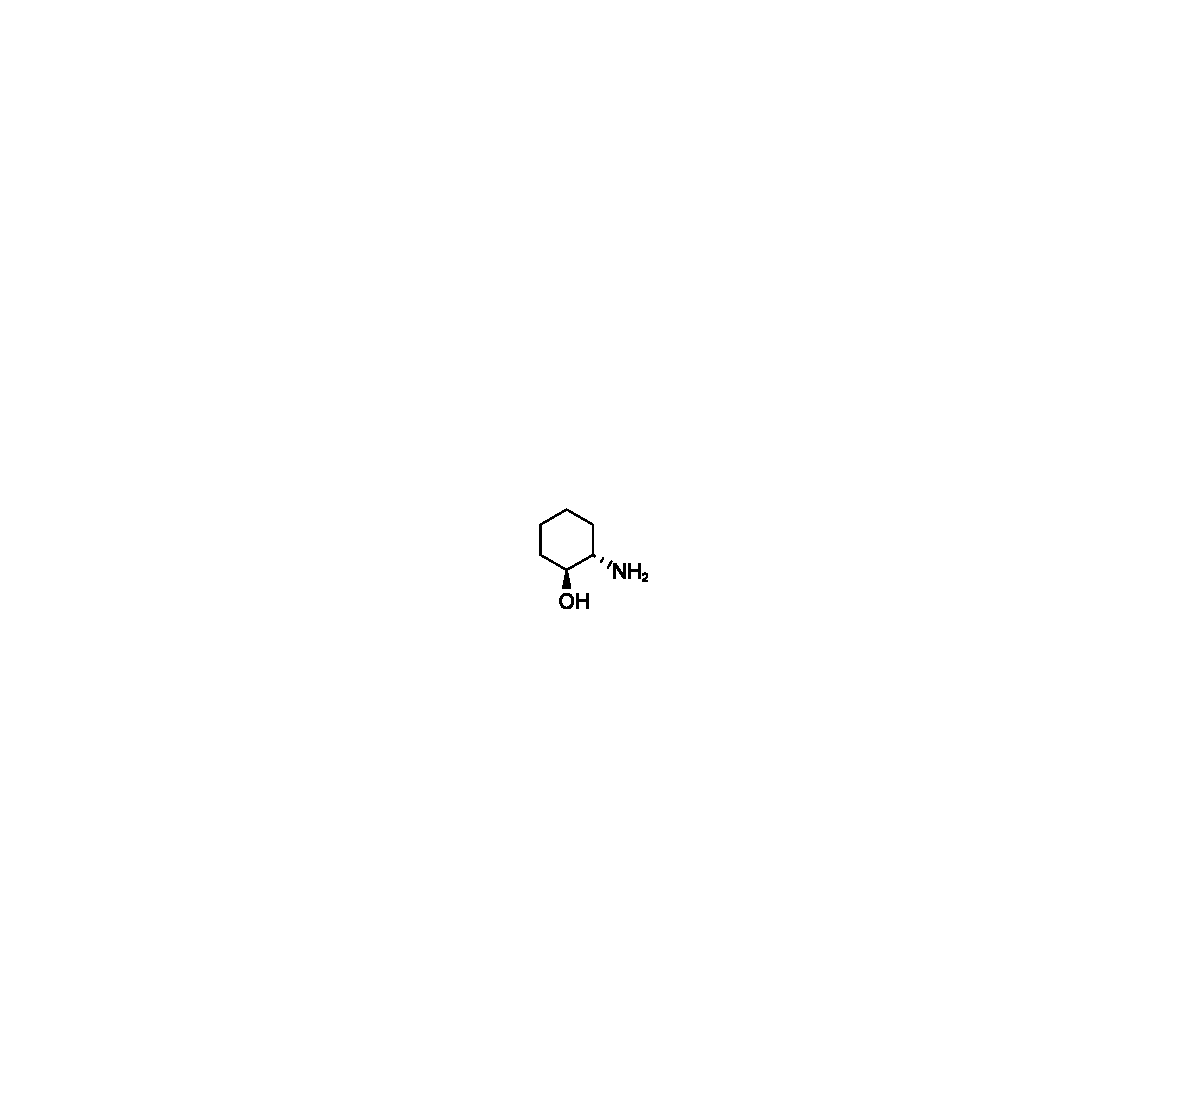
\includegraphics[draft=false,scale=1]{HOcy6NH2.eps}
%	\end{center}
%\end{scheme}
%
%4-chloro-N-((trans)-2-hydroxycyclohexyl)butanamide  \compound{cmpd:HOcy6NH4Cl}
%
%%%LMO-3-010 (ugh at purification), LMO-3-014 (worked?)
%
%\begin{scheme}[H]
%	\begin{center}
%		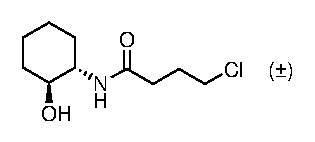
\includegraphics[scale=1]{HOcy6NH4Cl.eps}
%	\end{center}
%\end{scheme}
%
%4-azido-N-((trans)-2-hydroxycyclohexyl)butanamide  \compound{cmpd:HOcy6NH4N3}
%
%%%LMO-3-012 (small, didn't purify), LMO-3-015 (done)
%
%\begin{scheme}[H]
%	\begin{center}
%		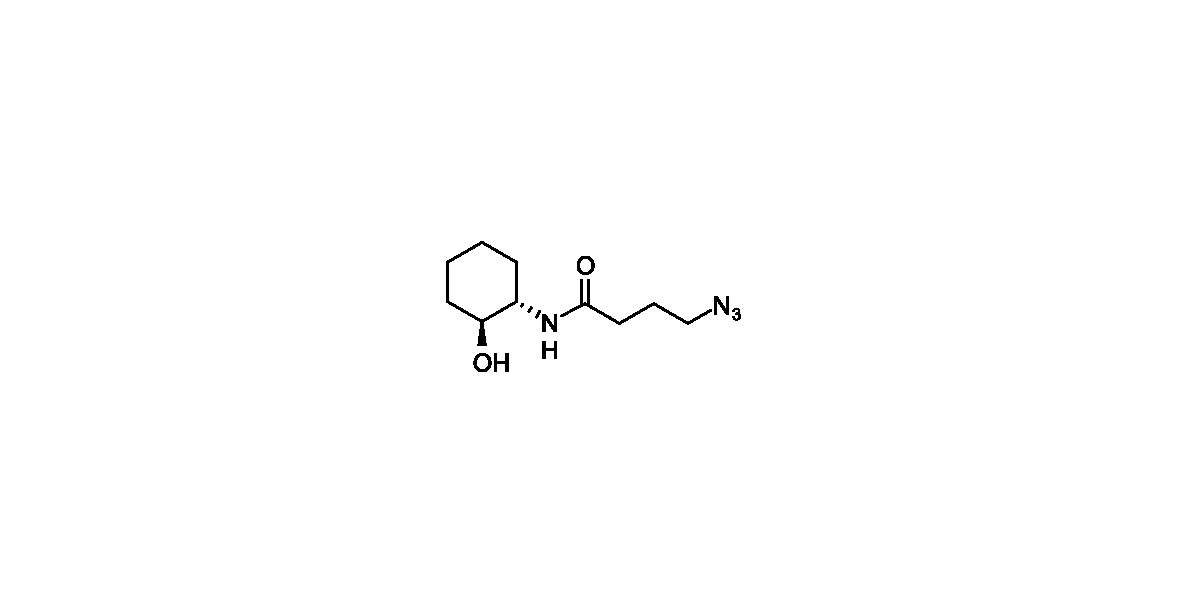
\includegraphics[scale=1]{HOcy6NH4N3.eps}
%	\end{center}
%\end{scheme}
%
%methyl 1-cyclopropyl-6-fluoro-7-(4-(4-(((trans)-2-hydroxycyclohexyl)amino)-4-oxobutyl)piperazin-1-yl)-4-oxo-1,4-dihydroquinoline-3-carboxylate \compound{cmpd:HOcy6NH4CipMe}
%
%%%LMO-3-013 (done)
%
%methyl 1-cyclopropyl-6-fluoro-4-oxo-7-(4-(4-oxo-4-((2-oxocyclohexyl)amino)butyl)piperazin-1-yl)-1,4-dihydroquinoline-3-carboxylate \compound{cmpd:Ocy6NH4CipMe}
%
%%%LMO-3-017 (done)
%
%1-cyclopropyl-6-fluoro-7-(4-(4-(1-(4-(((trans)-2-hydroxycyclohexyl)amino)-4-oxobutyl)-1H-1,2,3-triazol-4-yl)butyl)piperazin-1-yl)-4-oxo-1,4-dihydroquinoline-3-carboxylic acid \compound{cmpd:HOcy6NH4T4Cip}
%
%%%LMO-3-016 (done)
%
%1-cyclopropyl-6-fluoro-4-oxo-7-(4-(4-(1-(4-oxo-4-((2-oxocyclohexyl)amino)butyl)-1H-1,2,3-triazol-4-yl)butyl)piperazin-1-yl)-1,4-dihydroquinoline-3-carboxylic acid \compound{cmpd:Ocy6NH4T4Cip}
%
%%%LMO-3-018 (done? awaiting NMR)
%
%
%
%
%
%
%
%\subsection{(\textit{S})-1-Cyclopropyl-6-fluoro-4-oxo-7-(4-(4-(1-(4-oxo-2-((2-oxotetrahydrofuran-3-yl)amino)butyl)-1H-1,2,3-triazol-4-yl)butyl)piperazin-1-yl)-1,4-dihydroquinoline-3-carboxylic acid \compound{cmpd:HL4Y4Cip}}
%
%%notmade
%
%\begin{scheme}[H]
%	\begin{center}
%		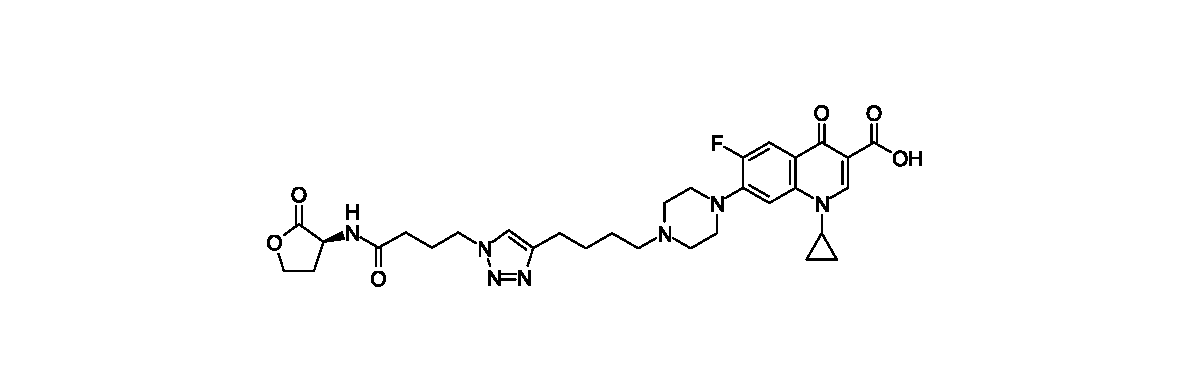
\includegraphics[scale=1]{HL4T4Cip}
%	\end{center}
%\end{scheme}
%
%
%\subsection{(\textit{S})-1-cyclopropyl-6-fluoro-4-oxo-7-(4-(4-(1-(6-oxo-6-((2-oxotetrahydrofuran-3-yl)amino)hexyl)-1H-1,2,3-triazol-4-yl)butyl)piperazin-1-yl)-1,4-dihydroquinoline-3-carboxylic acid \compound{cmpd:HL6Y4Cip}}
%
%%notmade
%
%\begin{scheme}[H]
%	\begin{center}
%		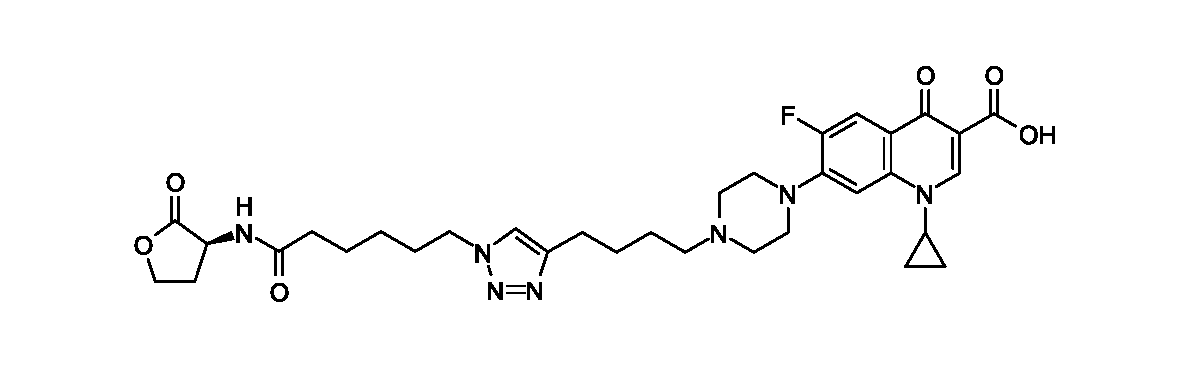
\includegraphics[scale=1]{HL6T4Cip}
%	\end{center}
%\end{scheme}
%
%
%\subsection{1-cyclopropyl-6-fluoro-7-(4-(4-(1-(2-heptyl-4-oxo-1,4-dihydroquinolin-6-yl)-1H-1,2,3-triazol-4-yl)butyl)piperazin-1-yl)-4-oxo-1,4-dihydroquinoline-3-carboxylic acid \compound{cmpd:azHHQY4Cip}}
%
%%notmade
%
%\begin{scheme}[H]
%	\begin{center}
%		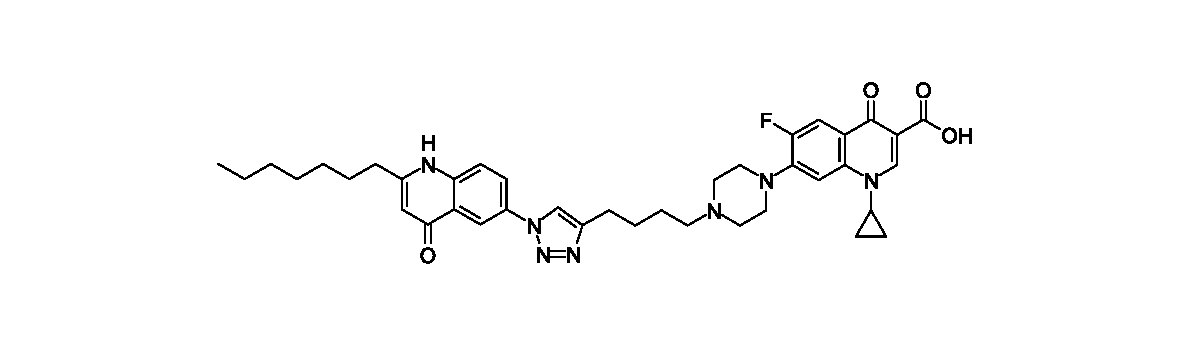
\includegraphics[scale=1]{6HHQT4Cip}
%	\end{center}
%\end{scheme}
%
%\subsection{1-cyclopropyl-6-fluoro-7-(4-(4-(1-(2-heptyl-3-hydroxy-4-oxo-1,4-dihydroquinolin-6-yl)-1H-1,2,3-triazol-4-yl)butyl)piperazin-1-yl)-4-oxo-1,4-dihydroquinoline-3-carboxylic acid \compound{cmpd:azPQSY4Cip}}
%
%%notmade
%
%\begin{scheme}[H]
%	\begin{center}
%		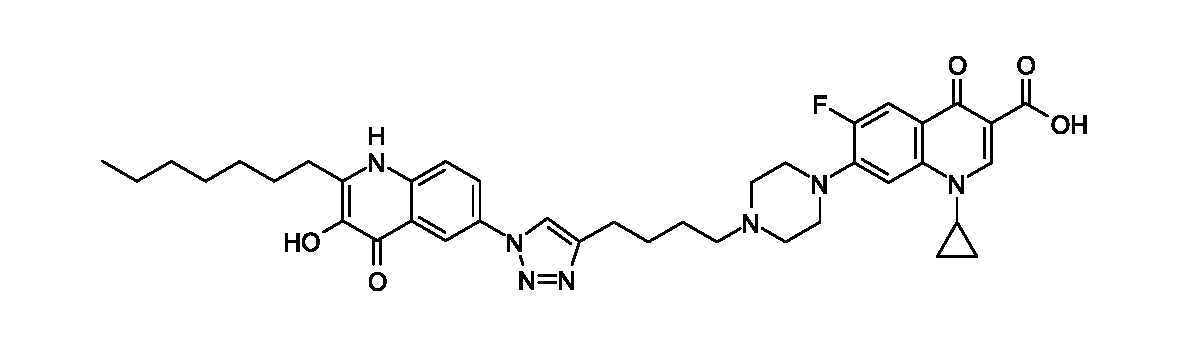
\includegraphics[scale=1]{6PQST4Cip}
%	\end{center}
%\end{scheme}
%
%\subsection{1-cyclopropyl-6-fluoro-4-oxo-7-(4-(4-(1-(6-(4-oxo-1,4-dihydroquinolin-2-yl)hexyl)-1H-1,2,3-triazol-4-yl)butyl)piperazin-1-yl)-1,4-dihydroquinoline-3-carboxylic acid \compound{cmpd:HHQazY4Cip}}
%
%%notmade
%
%\begin{scheme}[H]
%	\begin{center}
%		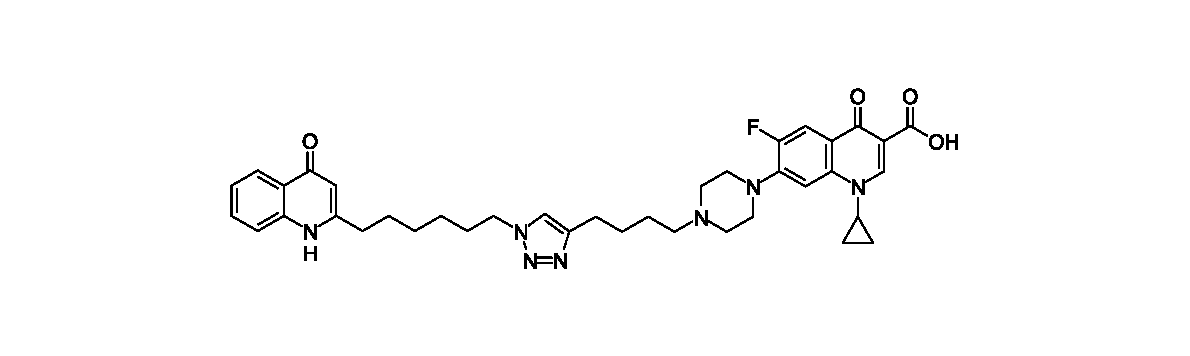
\includegraphics[scale=1]{HHQT4Cip}
%	\end{center}
%\end{scheme}
%
%\subsection{1-cyclopropyl-6-fluoro-7-(4-(4-(1-(6-(3-hydroxy-4-oxo-1,4-dihydroquinolin-2-yl)hexyl)-1H-1,2,3-triazol-4-yl)butyl)piperazin-1-yl)-4-oxo-1,4-dihydroquinoline-3-carboxylic acid \compound{cmpd:PQSazY4Cip}}
%
%%notmade
%
%\begin{scheme}[H]
%	\begin{center}
%		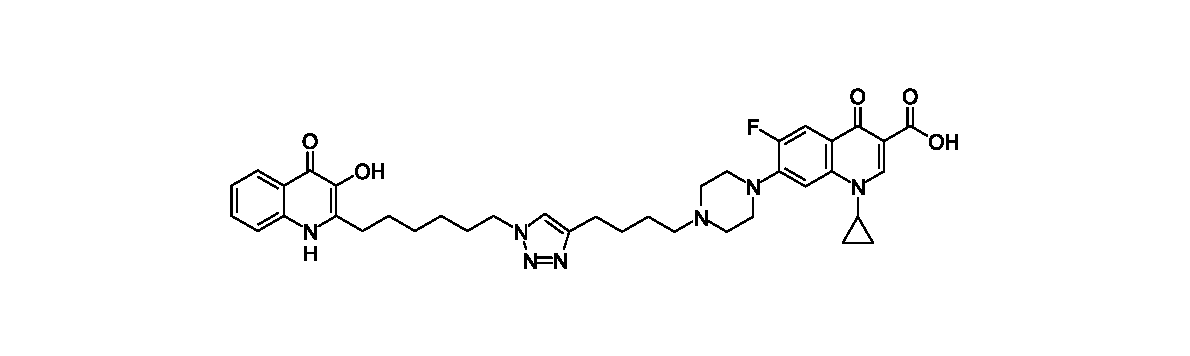
\includegraphics[scale=1]{PQST4Cip}
%	\end{center}
%\end{scheme}


%\subsection{(\textit{S})-1-Cyclopropyl-6-fluoro-4-oxo-7-(4-(4-(1-(4-oxo-2-((2-oxotetrahydrofuran-3-yl)amino)butyl)-1H-1,2,3-triazol-4-yl)butyl)piperazin-1-yl)-1,4-dihydroquinoline-3-carboxylic acid \compound{cmpd:HL4T4Tri}}
%
%\begin{scheme}[H]
%	\begin{center}
%		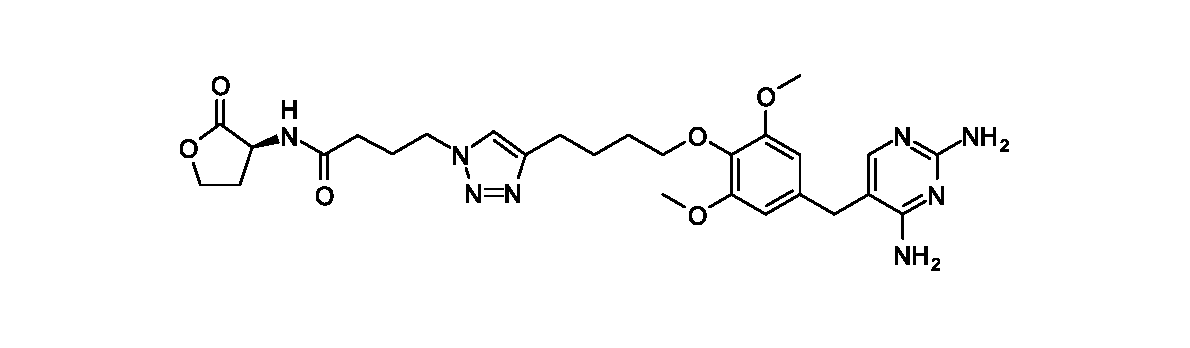
\includegraphics[scale=1]{HL4T4Tri}
%	\end{center}
%\end{scheme}